\documentclass[a4paper]{article} 
\addtolength{\hoffset}{-2.25cm}
\addtolength{\textwidth}{4.5cm}
\addtolength{\voffset}{-3.25cm}
\addtolength{\textheight}{5cm}
\setlength{\parskip}{0pt}
\setlength{\parindent}{0in}

\usepackage{blindtext} % Package to generate dummy text
\usepackage{charter} % Use the Charter font
\usepackage[utf8]{inputenc} % Use UTF-8 encoding
\usepackage{microtype} % Slightly tweak font spacing for aesthetics
\usepackage[english]{babel} % Language hyphenation and typographical rules
\usepackage{amsthm, amsmath, amssymb, amsfonts} % Mathematical typesetting
\usepackage{float} % Improved interface for floating objects
\usepackage[final, colorlinks = true, 
linkcolor = black, 
citecolor = black]{hyperref} % For hyperlinks in the PDF
\usepackage{graphicx, multicol} % Enhanced support for graphics
\usepackage{xcolor} % Driver-independent color extensions
\usepackage{marvosym, wasysym} % More symbols
\usepackage{rotating} % Rotation tools
\usepackage{subcaption}
\usepackage{wrapfig}
\usepackage{censor} % Facilities for controlling restricted text
\newcommand{\note}[1]{\marginpar{\scriptsize \textcolor{red}{#1}}} % Enables comments in red on margin
\usepackage{bm}
\usepackage{blkarray}
\usepackage{enumitem}
\usepackage{pgfplots}
\usepackage{tikz}

\newcommand{\pd}[2]{\frac{\partial #1}{\partial #2}}
\newcommand{\loss}[0]{\mathcal{L}}
\newcommand{\chain}[3]{\frac{\partial #1}{\partial #2}\frac{\partial #2}{\partial #3}}
\newcommand{\eq}[1]{\begin{equation*}\begin{split}#1\end{split}\end{equation*}}
\newcommand{\coderef}[0]{Please find the implementation in the folder with the code files.}
\newcommand{\TODO}[1]{\textbf{\textcolor{red}{#1}}}

\definecolor{green}{RGB}{0,160,0}
\definecolor{blue}{RGB}{0,0,160}
\definecolor{red}{RGB}{160,0,0}
\definecolor{orange}{RGB}{200,160,0}
\definecolor{purple}{RGB}{170,0,200}
\definecolor{cyan}{RGB}{0,200,200}
\definecolor{lightred}{RGB}{200,50,50}

\setcounter{tocdepth}{2}
% Title Page
\title{Summary Deep Learning}
\author{Phillip Lippe}


\begin{document}
\maketitle
\tableofcontents
\newpage

\section{Introduction}
\subsubsection{Perceptron}
\begin{itemize}
	\item Single perceptron weights every input with a weight, and adds a bias term
	\item Step function as output: if input sum greater zero, then output is 1, else 0 (or -1)
	\item Problem: can only learn linear problems and not e.g. XOR
	\item Overcoming by multi-layer perceptron 
\end{itemize}
\section{Modular Learning}
\begin{itemize}
	\item \textit{Definition}: A family of \textcolor{green}{parametric}, \textcolor{lightred}{non-linear} and \textcolor{blue}{hierarchical} \textcolor{orange}{representation learning functions}, which are \textcolor{red}{massively optimized with stochastic gradient descent} to \textcolor{purple}{encode domain knowledge}, i.e. domain invariances, stationarity.
	% \item Although with two-layer (shallow) network, we can approximate all possible functions, a deep architecture tends to be more efficient and generalize better
	\item A neural network is a series of hierarchically connected functions $\Rightarrow$ Directed Acyclic graph
	\item Note that it is not allowed to have loops except over time/additional dimension
\end{itemize}
\begin{figure}[ht!]
	\centering
	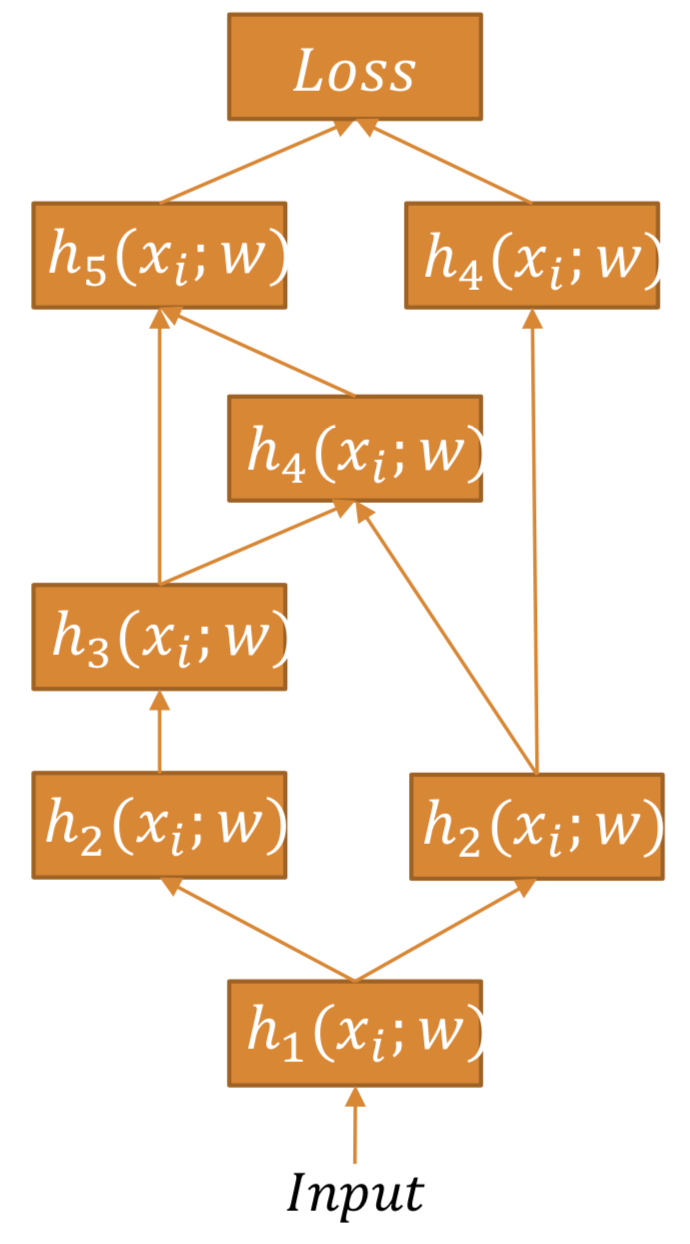
\includegraphics[width=0.2\textwidth]{figures/modularity_example_network.png}
	\caption{Example network with interweaved connections. The architecture can be made arbitrarily complex, and can also include recurrent connections.}
	\label{fig:modularity_example_network}
\end{figure}
\subsection{Module}
\begin{itemize}
	\item A module is the simplest mathematical component in a NN, and can be expressed by $a=h(x;w)$ where $a$ is the output, $x$ the input, $w$ trainable parameters and $h$ an activation function
	\item $w$ mostly learned by gradient-based methods, usually maximizing the likelihood
	\begin{itemize}
		\item ML solution: $w^{*} = \arg\max\limits_{w}\prod\limits_{x,y}p_{model}\left(y|x;w\right)$
		\item For gradient-based methods, we can minimize the negative log likelihood:\\ $\mathcal{L}(w) = -\mathbb{E}_{x,y\sim \tilde{p}_{data}}\left[\log p_{model}\left(y|x;w\right)\right]$
		\item If output is Gaussian, we would get the $\ell_2$ norm
		\item If output is Laplacian, we would get the $\ell_1$ norm
	\end{itemize} 
	\item Using a loss function that matches the output distribution of the network helps, because:
	\begin{itemize}
		\item It makes math simpler (exponential cancels out)
		\item Better numerical stability ($\log$ with very small/negative values, helps for e.g. Softmax+CrossEntropy)
		\item Makes gradients larger as exponential-like activations often lead to saturation, which means gradients are almost 0 (but not with $\log$)
	\end{itemize}
	\item It is important that the input and output distribution of every module match, as otherwise we get inconsistent behavior and makes it harder to learn
	\begin{itemize}
		\item For activation functions, this means we prefer them to be mostly activated around the origin and centered
		\item Otherwise, e.g. ReLU can be come a linear unit or set everything to 0
	\end{itemize}
\end{itemize}
\subsubsection{Example modules}
\begin{itemize}
	\item \textbf{Linear module}: $a = wx$
	\begin{itemize}
		\item Simple gradients $\frac{\partial a}{\partial w} = x$, $\frac{\partial a}{\partial x} = w$
		\item No activation saturation $\Rightarrow$ strong, reliable gradients
	\end{itemize}
	\item \textbf{Rectified Linear Unit}: $a = \max(0,x)$
	\begin{itemize}
		\item Gradient is step function. $\pd{a}{x} = \begin{cases}
		0 & \text{ if } x\leq 0\\
		1 & \text{ if } x > 0\\
		\end{cases}$
		\item Hence, strong, fast gradients
		\item However, dead neurons might be an issue when initialization/weights produce outputs smaller 0 for every input 
		\item Different variations like LeakyReLU, Softplus ($\ln(1+e^{x})$), NoisyReLU exist
	\end{itemize}
	\item \textbf{Sigmoid}: $a=\sigma(x)=\frac{1}{1+e^{-x}}$
	\begin{itemize}
		\item Gradient easy to calculate: $\pd{a}{x} = \sigma(x)\left(1-\sigma\left(x\right)\right)$
		\item Can be used as output function for probability distribution between $[0,1]$
		\item Saturates and has small gradients
		\item Not centered around origin $\Rightarrow$ not good choice for within a network
	\end{itemize}
	\item \textbf{Tanh}: $a=\tanh\left(x\right)=\frac{e^{x}-e^{-x}}{e^{x}+e^{-x}}$
	\begin{itemize}
		\item Gradients $\pd{a}{x}=1-\tanh\left(x\right)^2$
		\item Saturates as well, but has slightly higher gradients than sigmoid and is centered around origin
	\end{itemize}
	\item \textbf{Softmax}: $a^{(k)} = \text{softmax}\left(x^{(k)}\right) = \frac{e^{x^{(k)}}}{\sum_j e^{x^{(j)}}}$
	\begin{itemize}
		\item Probability distribution over multiple classes
		\item Softmax trick for numerical stability: $\frac{e^{x^{(k)}-\mu}}{\sum_j e^{x^{(j)}-\mu}}$
	\end{itemize}
\end{itemize}
\subsection{Backpropagation}
\begin{itemize}
	\item Calculate gradients of all parameters in the network based on the loss on the last layer
	\item Principle of chain rule: $\pd{z}{x} = \sum_j \chain{z}{y_i}{x}$ (gradients from all possible paths)
	\begin{itemize}
		\item In vector notation: $\nabla_{\bm{x}} \bm{z} = \left(\pd{\bm{y}}{\bm{x}}\right)^T \cdot \nabla_{\bm{y}} \bm{z}$ with Jacobian $\pd{\bm{y}}{\bm{x}} = \left[\begin{array}{ccc}
		\pd{y_1}{x_1} & \pd{y_1}{x_2} & \pd{y_1}{x_3} \\[5pt]
		\pd{y_2}{x_1} & \pd{y_2}{x_2} & \pd{y_2}{x_3} \\
		\end{array}\right]$
	\end{itemize}
	\item Steps of Backpropagation:
	\begin{enumerate}
		\item Compute forward propagations for all layers recursively:
		$a^{(l)} = h^{(l)}\left(x^{(l)}\right) \text{ and } x^{(l+1)} = a^{(l)}$
		\item Compute the reverse path. 
		$$\pd{\mathcal{L}}{a^{(l)}} = \left(\pd{a^{(l+1)}}{x^{(l+1)}}\right)^T \cdot \pd{\mathcal{L}}{a^{(l+1)}}, \hspace{4mm} \pd{\mathcal{L}}{\theta^{(l)}} = \pd{a^{(l)}}{\theta^{(l)}} \cdot \left(\pd{\mathcal{L}}{a^{(l)}}\right)^T$$
		\item Use gradients $\pd{\mathcal{L}}{\theta^{(l)}}$ to update parameters via SGD
	\end{enumerate}
\end{itemize}
\section{Deep Learning Optimizations}
\begin{itemize}
	\item Pure optimization has a very direct goal, namely finding the optimum. However, in Machine Learning, we define a training goal. Thus, the ``optimal'' parameters might not necessarily be the optimum (e.g. overfitting)
\end{itemize}
\subsection{Stochastic Gradient Descent}
\begin{itemize}
	\item Pushing the weights towards highest gradient change
	$$w_{t+1} = w_{t} - \eta_t \nabla_{w} \mathcal{L}$$
	\item \textit{Gradient descent}: gradients on the full dataset. However:
	\begin{itemize}
		\item Dataset is mostly too large for this
		\item No real guarantee that this leads to a good optimum and/or it will converge faster
	\end{itemize}
	\item \textit{Stochastic gradient descent}: approximate gradients by averaging over a small batch. 
	\begin{itemize}
		\item Standard error is inverse proportional to number of elements $m$ in a batch: $\sigma / \sqrt{m}$.
		\item Noisy gradients help to escape local minima, acts as regularization
		\item Does sample roughly representative gradients from dataset. Is better as training data is also just a rough approximation of what the test data might look like (optimum on training $\neq$ optimum on test)
		\item SGD is faster, especially in first iterations
		\item SGD is able to adapt with dynamically changing datasets
	\end{itemize}
	\item \textit{Ill conditioning}: if gradients are large, applying them can lead to worse performance. This is the case if the second order derivative changes faster 
\end{itemize}
\subsection{Advanced optimizations}
\subsubsection{Gradient-based optimization}
\begin{itemize}
	\item \textit{Pathological curvatures}: move through a ravine towards minimum. SGD tends to oscillate between the walls because they have high gradients
	\begin{itemize}
		\item Second order optimization can help a lot for pathological curvatures: $$w_{t+1} = w_{t} - H_{\mathcal{L}}^{-1} \eta_t g_t$$
		\item Hessian $H_{\mathcal{L}}^{ij} = \pd{\mathcal{L}}{w_i\partial w_j}$ works as adaptive learning rate per parameter
		\item However, unfeasible in practice because Hessian gets very large
	\end{itemize}
	\begin{figure}[ht!]
		\centering
		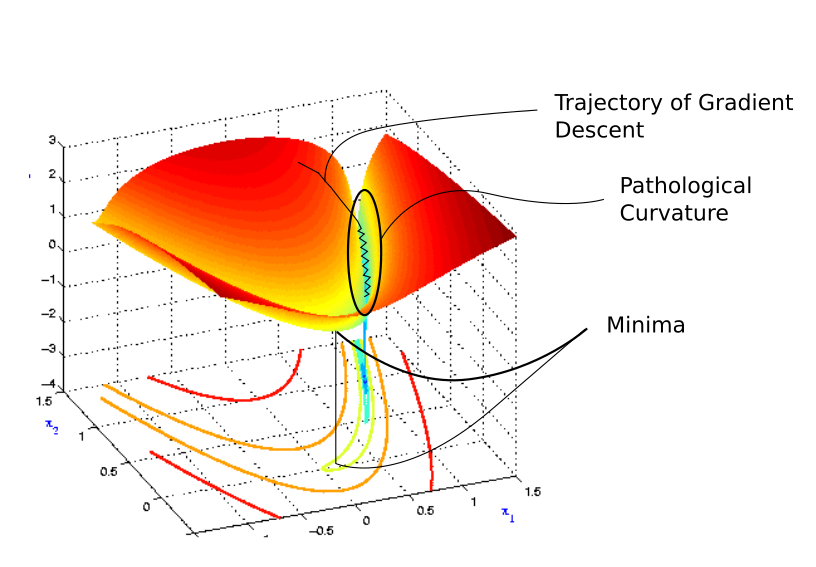
\includegraphics[width=0.3\textwidth]{figures/optimization_pathological_curvatures.png}
		\caption{Pathological curvature}
		\label{fig:optimization_pathological_curvatures}
	\end{figure}
	\item \textbf{Momentum}: maintain \textit{momentum} from previous parameter updates to dampen the oscillations.
	\begin{equation*}
		\begin{split}
			u_{t+1} & = \gamma u_{t} - \eta_t g_t \\
			w_{t+1} & = w_{t} + u_{t+1}
		\end{split}
	\end{equation*}
	\begin{itemize}
		\item Works as a exponential averaging $\Rightarrow$ more robust gradients, faster convergence
		\item $\gamma$ might be initialized lower and then increased over time to $0.9$
		\item Standard values for $\gamma$ are between $0.5$ and $0.9$ (note that a lower learning rate should be used compared to standard SGD)
	\end{itemize}
	\item \textbf{RMSprop}: adapting learning rate on current loss surface.
	\begin{equation*}
		\begin{split}
			r_t & = \alpha \cdot r_{t-1} + \left(1 - \alpha\right) \cdot g_t^2\\
			\eta_t & = \frac{\eta}{\sqrt{r_t} + \epsilon} \\
			w_{t+1} & = w_{t} - \eta_t \cdot g_t\\
		\end{split}
	\end{equation*}
	\begin{itemize}
		\item $r_t$ is the (exponentially) averaged gradient norm describing the size of the gradients (per dimension!)
		\item The learning rate is then adapted by $\eta_t$ at every time step for each dimension independently
		\item $\epsilon$ to prevent numerical instability and too large learning rates
		\item With the adapted learning rate, we update our weights with SGD
	\end{itemize}
	\item \textbf{Adam}: Combining adaptive learning rate and momentum
	\begin{equation*}
		\begin{split}
			m^{(t)} & = \beta_1 m^{(t-1)} + (1 - \beta_1)\cdot g^{(t)}\\
			v^{(t)} & = \beta_2 v^{(t-1)} + (1 - \beta_2)\cdot \left(g^{(t)}\right)^2\\
			\hat{m}^{(t)} & = \frac{m^{(t)}}{1-\beta^{t}_1}, \hat{v}^{(t)} = \frac{v^{(t)}}{1-\beta^{t}_2}\\
			w^{(t)} & = w^{(t-1)} - \frac{\eta}{\sqrt{v^{(t)}} + \epsilon}\circ \hat{m}^{(t)}\\
		\end{split}
	\end{equation*}
	\begin{itemize}
		\item Keeps track of the gradient norm for momentum $m^{(t)}$, and norm (also known as velocity) $v^{(t)}$
		\item The hyperparameters $\beta_1$ and $\beta_2$ correlate with the $\gamma$ and $\alpha$ respectively from the previous approaches
		\item The adaptive learning rate is expressed by $\hat{v}^{(t)}$, and the exponentially averaged gradients by $\hat{m}^{(t)}$
		\item The division is to remove the bias of $m^{(0)}$ and $v^{(0)}$ being zero. Note that $\beta_1^t$ means the value of $\beta_1$ to the power $t$, and not at time step $t$
		\item Adam is in general better for complex models, but might fail on easy/stupid tasks compared to simple methods like SGD
	\end{itemize}
	\item \textbf{Adagrad}: adapting learning rate based on both gradient scale and frequency of updates
	\begin{equation*}
		\begin{split}
			G_t & = G_{t-1} + \text{diag}\left(g_t^2\right)\\
			w_{t+1} & = w_{t} - \frac{\eta}{\sqrt{G_t + \epsilon}}\cdot g_t\\
		\end{split}
	\end{equation*}
	\begin{itemize}
		\item Very similar to RMSprop, but sums the scales over all time steps ($G_t$) instead of exponentially averaging 
		\item Less sensitive to learning rate tuning, but it gets very small over training time annealing to 0
	\end{itemize} 
	\item \textbf{Nesterov momentum}: use the future gradient instead of the current gradient. Leads to better convergence in theory
\end{itemize}
\subsubsection{Bayesian optimization}
\begin{itemize}
	\item Gradient-based optimizations have the problem of getting stuck in local minima
	\item Bayesian optimization is a gradient-free, educated trial and error guesser that works in lower dimensional spaces (up to 1000, but mostly 20 to 50 parameters)
	\item Determines the next point/parameter values to evaluate based on variance/uncertainty, and expected/predictive value. 
	\item Can be used for e.g. network architecture search
\end{itemize}
\subsection{Normalization}
\begin{itemize}
	\item Data pre-processing
	\begin{itemize}
		\item Center data around 0 (activation functions are designed for that)
		\item Scale input variables to have similar diagonal covariances (not if features are differently important)
		\item De-correlate features if there is no inductive bias (e.g. sequence over time)
	\end{itemize}
	\item \textbf{Batch normalization}: ensure Gaussian distribution of features over batches at every module input
	\begin{equation*}
		\begin{split}
			\mu_B = \frac{1}{m} \sum\limits_{i=1}^{m} x_i, &\hspace{5mm} \sigma_B^2 = \frac{1}{m} \sum\limits_{i=1}^{m} \left(x_i - \mu_B\right)^2 \\
			\hat{x}_i & = \frac{x_i - \mu_B}{\sqrt{\sigma^2 + \epsilon}} \\
			\hat{y}_i & = \gamma \cdot \hat{x}_i + \beta
		\end{split}
	\end{equation*}
	\begin{itemize}
		\item Normalize feature to $\hat{x}_i \sim \mathcal{N}(0,1)$, then rescale with trainable parameters $\gamma$ (variance) and $\beta$ (mean).
		\item Helps the optimizer to control mean and variance of input distribution, and reduces effects of 2nd order between layers $\Rightarrow$ easier, faster learning 
		\item Acts as regularizer as distribution depends on mini-batch and therefore introduces noise
		\item During testing, take a moving average of the last training steps and use those for $\mu_B$ and $\sigma_B^2$
	\end{itemize}
\end{itemize}
\subsection{Regularization}
\begin{itemize}
	\item Weight regularization needed to prevent overfitting
	\item \textbf{$\ell_2$-regularization}: Introduce objective term for minimizing weights
	$$w^{*}=\arg\min_w \mathcal{L} + \frac{\lambda}{2}\sum_l ||w_l||^2$$
	\begin{itemize}
		\item When using simple (stochastic) gradient descend, then $\ell_2$ regularization is the same as weight decay: $$w_{t+1} = \left(1-\lambda \eta_t\right) w_{t} - \eta_t \nabla_{\theta} \mathcal{L}$$
	\end{itemize}
	\item \textbf{$\ell_1$-regularization}: use $\ell_1$ objective, introduces sparse weights
	$$w^{*}=\arg\min_w \mathcal{L} + \lambda \sum_l ||w_l||$$
	\item \textbf{Early stopping}: stop the training when test error increases but training loss continues to decrease. Can be counted to regularization as training steps are reduced
	\item \textbf{Dropout}: setting activations randomly to 0 during training with probability $p$ (mostly between $0.1$ and $0.5$)
	\begin{itemize}
		\item During test time, every activation is reweighted by $1 - p$
		\item Reduces co-adaptations/-dependencies between neurons because none can solely depend on the other
		\item Neurons get more robust $\Rightarrow$ reduces overfitting
		\item Effectively, a different network architecture is used every iteration. Testing can be seen as using model ensemble
	\end{itemize}
\end{itemize}
\subsection{Weight initialization}
\begin{itemize}
	\item There are two forces on the weight magnitude: small weights are needed to keep data around origin, but large weights are required to have strong learning signals
	\item Initialization should preserve variance of activations (input variance $\approx$ output variance to keep distribution between modules same)
	\item Depends on non-linearity and data normalization
	\item \textbf{Xavier initialization}: to maintain data variance, the variance of the weights must be $1/d$ where $d$ is number of input neurons $\Rightarrow$ sample weight values from $w\sim\mathcal{N}(0,\sqrt{1/d})$
	\item \textbf{Initialization for ReLU}: ReLU set half of the output neurons to 0 $\Rightarrow$ double the weight variance to compensate zero flat-area: $w\sim\mathcal{N}(0,\sqrt{2/d})$
\end{itemize}
\section{Convolutional Neural Networks}
\begin{itemize}
	\item Images are stationary signals with spatial structure and huge dimensionality
	\item Input dimensions are highly correlated (e.g. translation invariant)
	\item Preserve spatial structure by convolutional filters, local connectivity (with shared weights) and being robust to local variances by spatial pooling
\end{itemize}
\subsection{Transfer Learning}
\begin{itemize}
	\item Use large datasets like ImageNet to learn useful features for other, smaller datasets
	\item Prevent overfitting, even for large networks
	\item Alternatively, we could also use a pre-trained network on task 1 as feature extractor for task 2 (same as freezing first layers)
	\item Which layer(s) to fine-tune?
	\begin{itemize}
		\item If both task have the same labels, we can initialize all layers. Otherwise, the classification layer (last layer) must be newly trained. If there is only very few data available, only fine-tune this layer
		\item If datasets are very different, the fully connected layers need to be replaced
		\item First convolutional filters capture low-level information that mostly does not change over datasets. Mid-level convolutions can be fine-tuned if dataset is large enough
	\end{itemize}
	\item Use a smaller learning rate for pre-initialized layers as network starts already from a point close to the optimum. New layers can be trained with higher learning rate
\end{itemize}
\subsection{Standard classification architectures}
\subsubsection{VGGNet}
\begin{itemize}
	\item All filter sizes are $3\times 3$, as this is the smallest filter size, and is more parameter efficient to build up large filters, plus additional non-linearity between filters
	\item $1\times 1$ convolutions used to increase non-linearity/complexity without increasing receptive field
\end{itemize}
\begin{figure}[ht!]
	\centering
	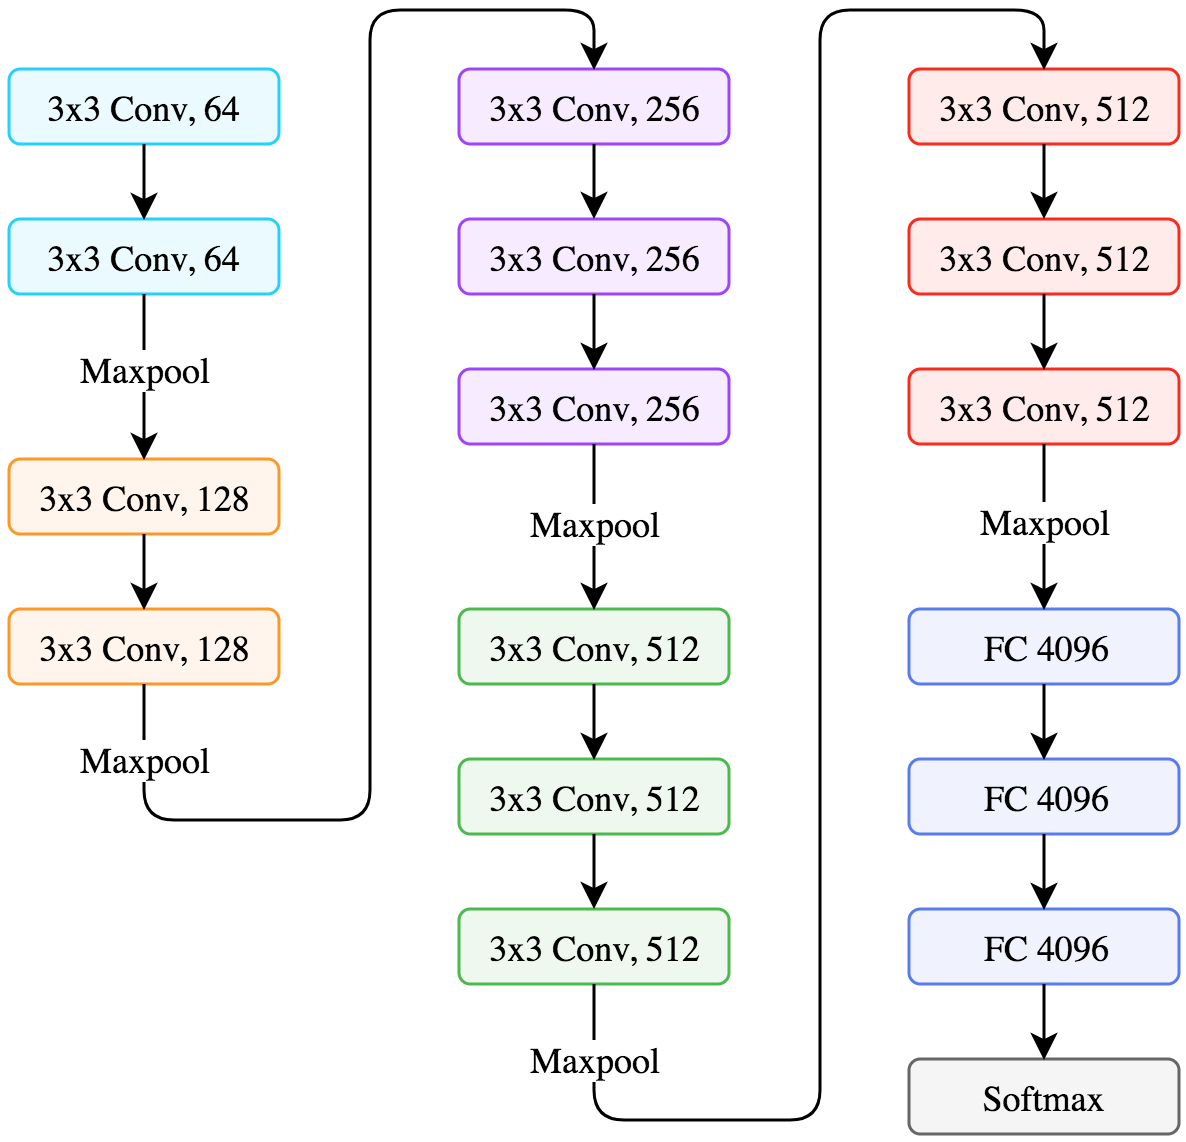
\includegraphics[width=0.3\textwidth]{figures/CNN_VGGnet.png}
	\caption{VGG16 architecture}
	\label{fig:CNN_VVGnet}
\end{figure}
\subsubsection{Inception}
\begin{itemize}
	\item Receptive fields should vary in size as objects can appear in different scales
	\item Naively stacking more convolutional operations on top of each other is expensive and prone to overfitting
	\item Inception module applies different filter sizes on same input ($1\times 1$ convolutions for feature reduction)
	\item Architecture consists of 9 Inception blocks
	\item Solution for vanishing gradients: have intermediate classifiers that amplify the gradient signal for early layers
	\item InceptionV2: $5\times 5$ replaced by two $3\times 3$ filters
	\item InceptionV3: $1\times 3$ and $3\times 1$ filters instead of $3\times 3$
	\item BatchNormalization has shown to be very helpful in this architecture
\end{itemize}
\begin{figure}[ht!]
	\centering
	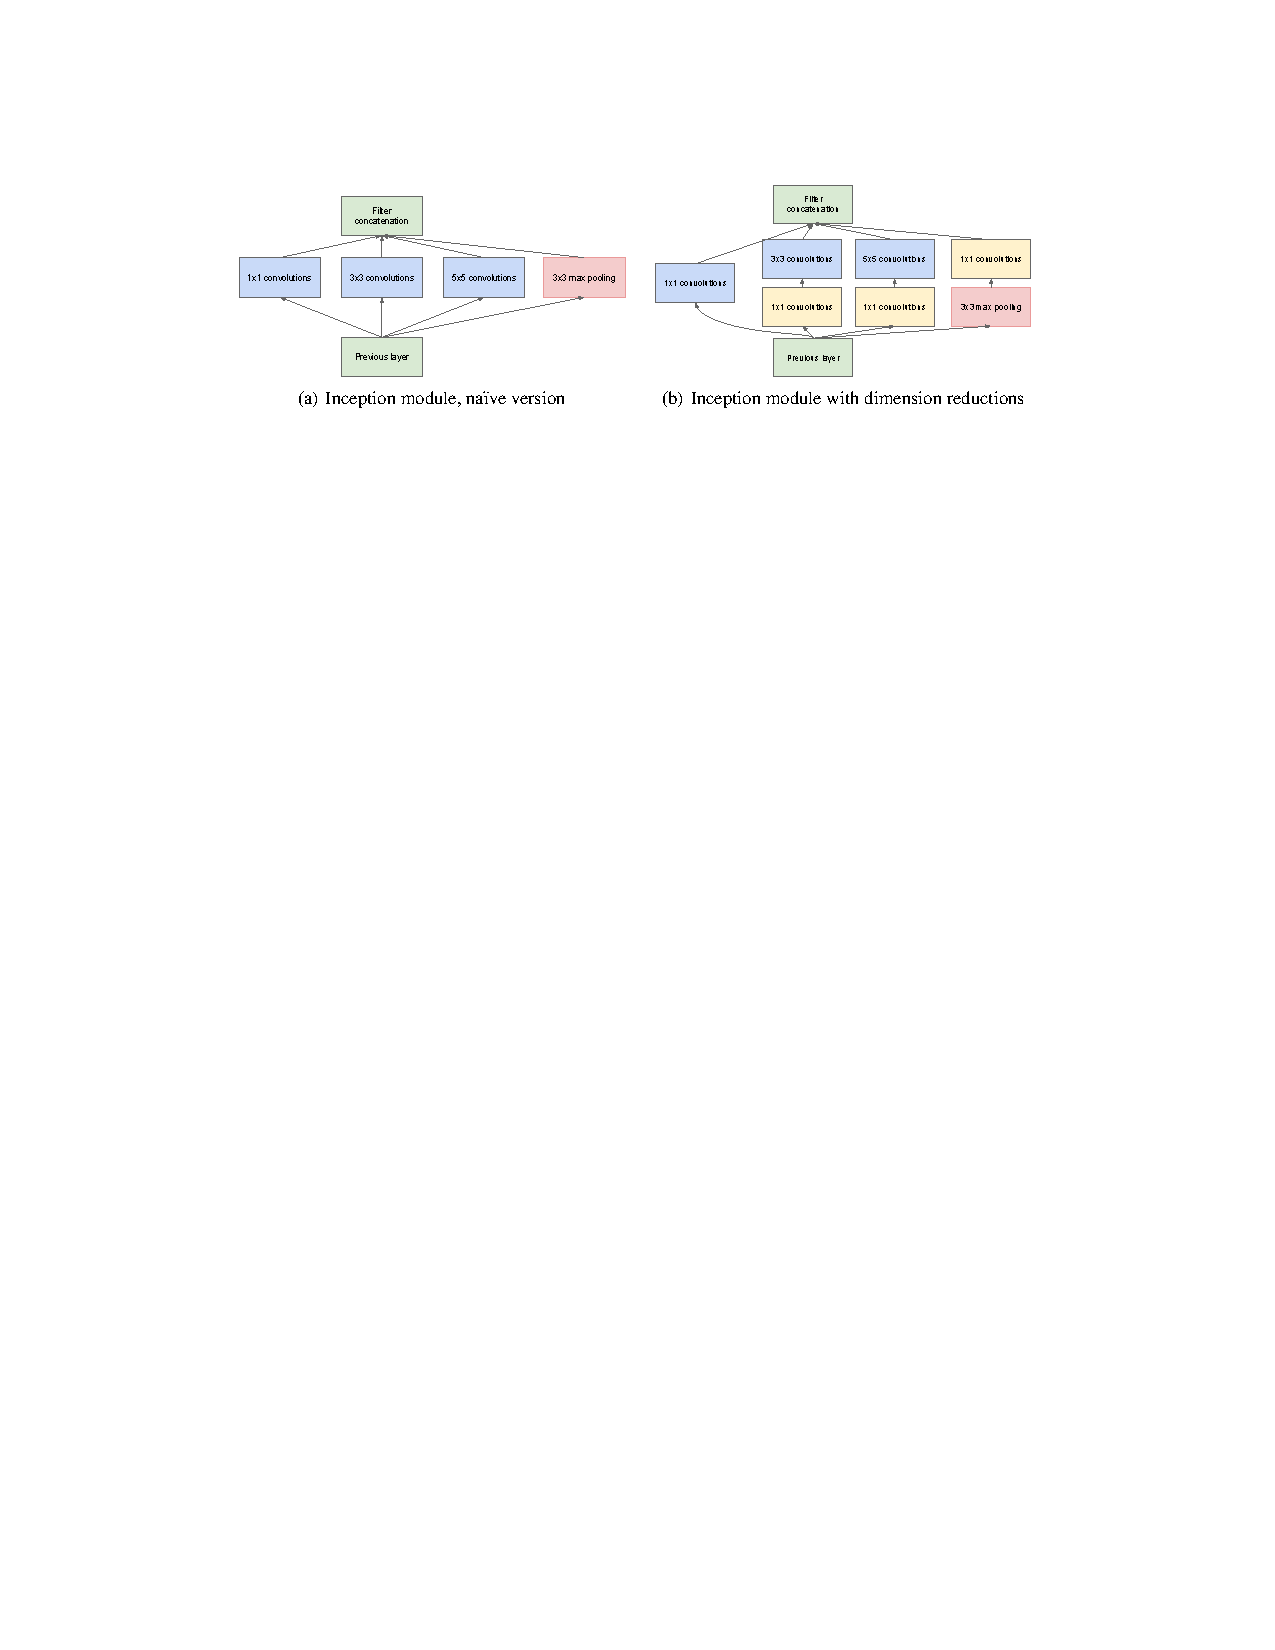
\includegraphics[width=0.8\textwidth]{figures/CNN_Inception_module.pdf}
	\caption{Inception module}
	\label{fig:CNN_Inception_module}
\end{figure}
\subsubsection{ResNet/DenseNet/HighwayNet}
\begin{itemize}
	\item Deeper networks are harder to optimize, and might actually achieve worse results than shallow ones because of that (although learning identity in additional layers must lead to same results)
	\item Better approach: try to model the difference that is learned in every layer $H(x) = F(x) + x$
	\item Different ways for modeling $F(x)$. Most popular ones shown in Figure~\ref{fig:CNN_ResNet_blocks}. BatchNormalization has been shown to be very important because of vanishing gradients
	\begin{figure}[ht!]
		\centering
		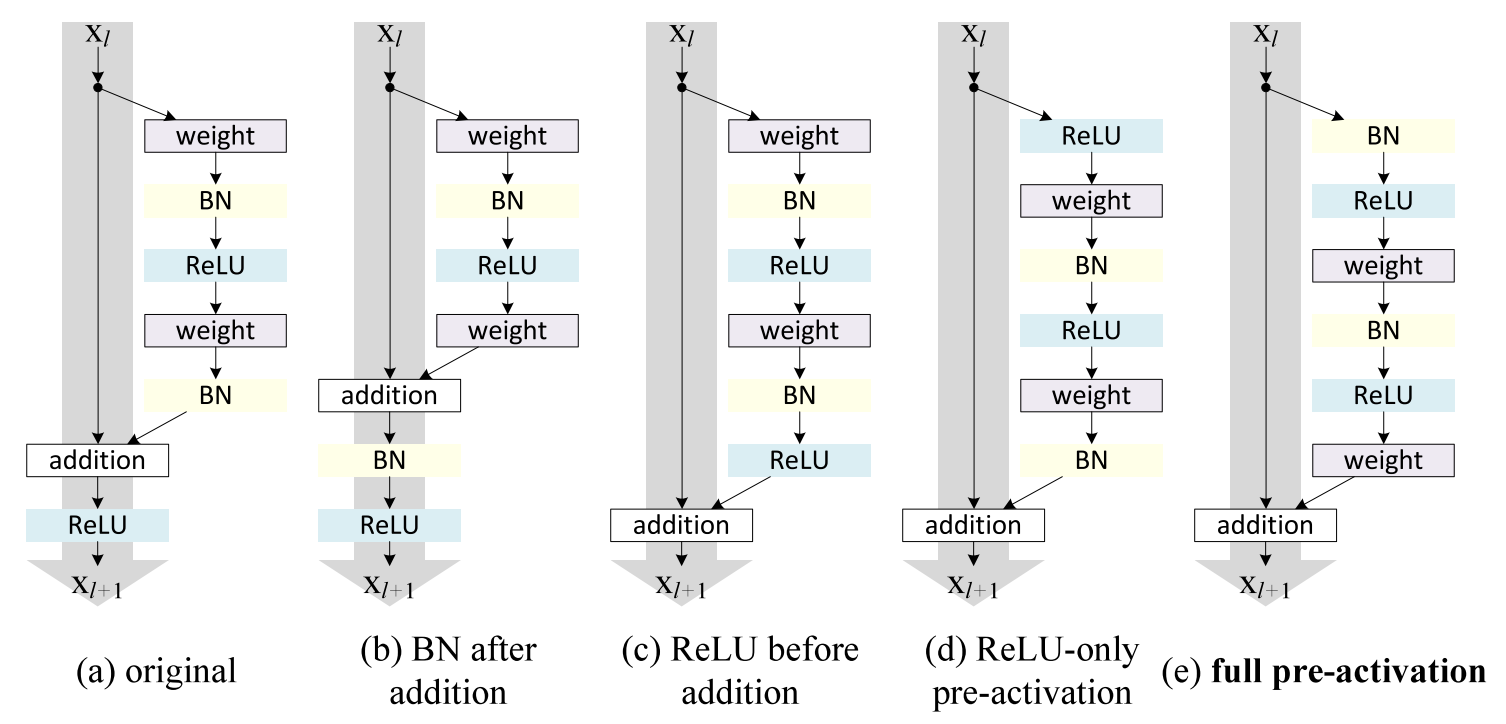
\includegraphics[width=0.7\textwidth]{figures/CNN_ResNet_blocks.png}
		\caption{ResNet blocks}
		\label{fig:CNN_ResNet_blocks}
	\end{figure}
	\item \textbf{HighwayNet} introduces a gate with learnable parameters to determine the importance of a layer: $H(x) = F(x) \cdot T(x) + x \cdot \left(1 - T\left(x\right)\right)$
	\item \textbf{DenseNet} uses skip connections to multiple forward layers. Creates complex blocks where last layer sees the input of all previous layers
\end{itemize}
\subsection{Tracking/Object detection}
\subsubsection{Fast R-CNN}
\begin{itemize}
	\item Based on middle feature map, get bounding boxes by e.g. selective search 
	\item RoI pooling returns fixed size feature map for selected bounding box (puts e.g. $3\times 3$ mask on features and pools accordingly)
	\item Features used to generate class prediction and location correction
	\item During training, sample multiple candidate boxes from image and train on all of them. Makes it more efficient/faster, \textit{but} batch elements might be highly correlated (in the paper, they report that they experienced it to be neglectable)
	\item Very accurate and fast, but external box proposals needed
	\item \textbf{Faster R-CNN}: train network to propose box locations
\end{itemize}
\subsubsection{Siamese Network for Training}
\begin{itemize}
	\item Use Siamese network to compare similarity of two patches
	\item If we compare patches over time, we can find objects with the highest similarity $\Rightarrow$ tracking of objects
	\item Can be trained on rich video dataset, and can be applied to unseen categories/targets
\end{itemize}
\subsection{Spatial Transformer Network}
\begin{itemize}
	\item ConvNets must be invariant/robust to pose/geometry changes. One simple way of doing it is data augmentation
	\item Better: use spatial transformer network to learn rotation/scale transformation
	\item Define grid on input. Scale, translation and rotation parameters are learned by the network and depend on the input. Finally, transform image based on the changed grid. 
	\item Operation is differentiable and thus can be learned
\end{itemize}
\section{Recurrent and Graph Neural Networks}
\subsection{Backpropagation through time}
\begin{itemize}
	\item Sequences are of arbitrary length. Standard networks like CNN mostly work on fixed input dimensionality
	\item Usage of memory with shared weights $\theta$: $$c_{t+1} = h_{\theta}\left(x_{t+1}, c_{t}\right) = h_{\theta}\left(x_{t+1}, h_{\theta}\left(x_{t}, c_{t-1}\right)\right) = ...$$
	\item Simple RNN cell: 
	\begin{equation*}
		\begin{split}
			c_t & = \tanh\left(U\cdot x_t + W \cdot c_{t-1}\right) \\
			y_t & = \text{softmax}\left(V \cdot c_{t}\right) \\
			\loss & = \sum\limits_{t=1}^{T} y_t^{*} \log y_t \\
		\end{split}
	\end{equation*}
	\item Gradient for output weights $V$:
	\begin{equation*}
		\begin{split}
			\pd{\loss_t}{V} & = \chain{\loss_t}{y_t}{c_t}\pd{c_t}{V} = \left(y_t - y_t^{*}\right) \cdot \left(c_t\right)^T\\
			\pd{\loss}{V} & = \sum\limits_{t=1}^{T} \pd{\loss_t}{V}\\
		\end{split}
	\end{equation*}
	\item Gradient for memory weights $W$: 
	\begin{equation*}
		\begin{split}
			\pd{\loss_t}{W} & = \chain{\loss_t}{y_t}{c_t}\pd{c_t}{W}\\
		\end{split}
	\end{equation*}
	\begin{itemize}
		\item In $\pd{c_t}{W}$, $c_t$ depends on $c_{t-1}$ which again depends on $W$. Thus, we have a recurrence in the gradient calculation:
		$$\pd{\loss_t}{W} = \sum\limits_{k=1}^{t} \chain{\loss_t}{y_t}{c_t}\chain{c_t}{c_k}{W}$$
		where $\pd{c_k}{W}$ only models the dependency exactly at time step $k$
		\item The gradient $\pd{c_t}{c_k}$ can be determined by the chain rule: $\pd{c_t}{c_k} = \prod\limits_{i=k+1}^{t} \pd{c_i}{c_{i-1}}$
		\item All in all, the final loss is:
		\begin{equation*}
			\begin{split}
				\pd{\loss}{W} & = \sum\limits_{t=1}^{T}\sum\limits_{k=1}^{t} \chain{\loss_t}{y_t}{c_t}\left(\prod\limits_{i=k+1}^{t} \pd{c_i}{c_{i-1}}\right)\pd{c_k}{W}
			\end{split}
		\end{equation*}
	\end{itemize}
	\item Gradient for input weights $U$ very similar to $W$: 
	\begin{equation*}
		\begin{split}
			\pd{\loss}{U} & = \sum\limits_{t=1}^{T}\sum\limits_{k=1}^{t} \chain{\loss_t}{y_t}{c_t}\left(\prod\limits_{i=k+1}^{t} \pd{c_i}{c_{i-1}}\right)\pd{c_k}{U}
		\end{split}
	\end{equation*}
	\item The problem with RNNs are that the gradients at time step $t$ depend on $c_{t-1}$ which also depends on $w$. However, the gradients are calculated with the assumption that $w$ stays the same for the previous time steps.
	\item This error can easily accumulate over many time steps so that in very long sequences, the gradients for the last steps are inaccurate
	\item Reduce learning rate/fewer updates, but this leads to slower training
\end{itemize}
\subsubsection{Vanishing gradients}
\begin{itemize}
	\item The exact derivations can be found in \href{http://proceedings.mlr.press/v28/pascanu13.pdf}{this paper}
	\item We assume an alternative formulation for simplicity here: $c_t = W \cdot \sigma(c_{t-1}) + U \cdot x_{t-1}$ where $\sigma$ is an arbitrary activation function. Then, the partial derivative between two time steps is\\ $\pd{c_{t}}{c_{k}} = \prod\limits_{i=k+1}^{t} \pd{c_{i}}{c_{i-1}} = \prod\limits_{i=k+1}^{t} W^T \cdot \text{diag}\left(\pd{\sigma\left(c_t\right)}{c_t}\right)$
	\item Hence, the magnitude of $\pd{c_{t+1}}{c_{t}}$ is bounded by this derivative: 
	$$\left\lVert \pd{c_{t+1}}{c_{t}}\right\rVert \leq \left\lVert W^T\right\rVert \cdot \left\lVert \text{diag}\left(\pd{\sigma\left(c_t\right)}{c_t}\right)\right\rVert$$
	\item In case the derivative of our non-linearity is bounded to a value $\gamma$ (which is 1 in case of tanh), we know that gradients vanish if the norm of the weight gradients are lower than $1/\gamma$:
	$$\left\lVert \pd{c_{t+1}}{c_{t}}\right\rVert \leq \left\lVert W^T\right\rVert \cdot \left\lVert \text{diag}\left(\pd{\sigma\left(c_t\right)}{c_t}\right)\right\rVert < \frac{1}{\gamma}\gamma = 1$$
	\item This term is exponentiated with the number of time steps. Thus, long sequences suffer even more of vanishing gradients $\Rightarrow$ learn only short-term relationships
	\item If however $\left\lVert \pd{c_{t+1}}{c_{t}}\right\rVert > 1$ because of $\left\lVert W^T\right\rVert \gg 1/\gamma$, then we can get exploding gradients
	\item Quick fix for exploding gradients: clip gradient norm. However, there the counterpart can happen where we only focus on long-term relationships
\end{itemize}
\subsubsection{Long Short-Term Memory}
\begin{itemize}
	\item Preventing vanishing gradients by gate mechanism
	\item By simply adding features to memory and limiting memory by sigmoid we can get strong gradients for any sequence length. Note that the gradients get lower in expectation because sigmoid has mean $0.5$. Nevertheless, if long-term dependencies are important, the network can learn them now
	\item \textit{Forget gate}: regulating how much information is kept from last time step
	\item \textit{Input + candidate gate}: Regulating which, and how much new information should be added given the current time step
	\item \textit{Output gate}: What features are important for the current time step
	\begin{figure}[ht!]
		\centering
		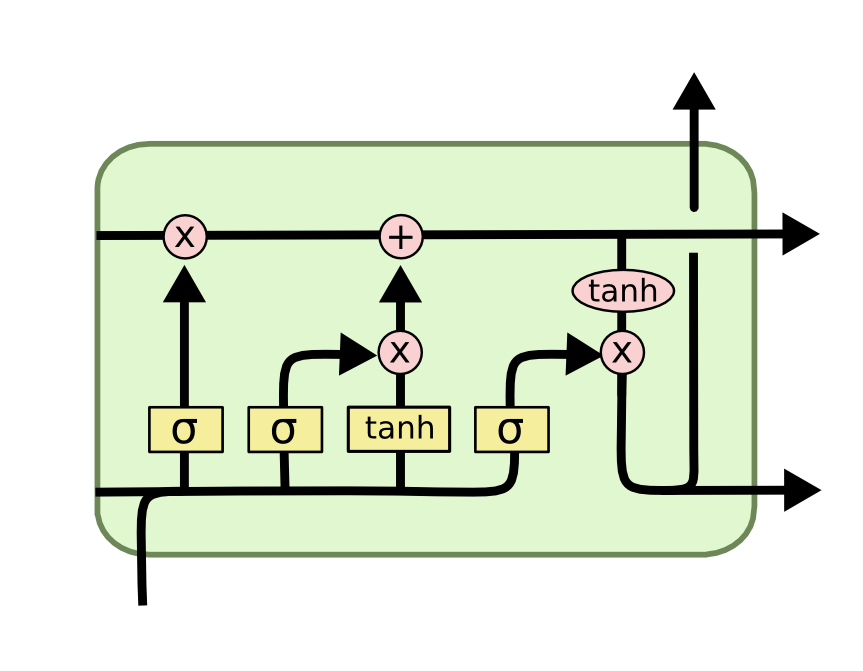
\includegraphics[width=0.3\textwidth]{figures/RNN_LSTM.png}
		\caption{Visualization of a LSTM cell}
		\label{fig:RNN_LSTM}
	\end{figure}
\end{itemize}
\subsection{Graph Neural Networks}
\begin{itemize}
	\item Perform operation on graph-structured data (e.g. social networks or knowledge graphs)
\end{itemize}
\subsubsection{Deep Walk}
\begin{itemize}
	\item Learning latent representations of vertices in a network
	\item The Deep Walk algorithm consists of two simple steps:
	\begin{enumerate}
		\item Perform random walks on the graph to generate node sequences
		\item Run skip-gram on sequence (with word window) to learn node embeddings
	\end{enumerate}
	\item \textit{Drawback}: algorithm has to be re-run if a new node is added, not useful for dynamic graphs
\end{itemize}
\subsubsection{GraphSage}
\begin{itemize}
	\item In every iteration, aggregate information of neighbors and the node itself to generate new embeddings
	\item Aggregation techniques are taking the mean (with weight and non-linearity applied on it afterwards), max pooling, or using a LSTM
\end{itemize}
\subsubsection{Graph Convolutional Networks}
\begin{itemize}
	\item A GNN layer takes as input the embeddings for every node $H^{(l)}$ and the adjacency matrix $A$, and create new embeddings $H^{(l+1)}$
	\item Graph convolutional layers use for this a matrix multiplication where weights are shared over nodes
	\item In the simplest form, a GCN layer can be defined as $h(H^{(l)}, A) = \sigma\left(A H^{(l)} W^{(l)}\right)$
	\item To make it more efficient, we add the identity matrix to $\hat{A} = A + I$ so that nodes use their old embeddings as well, and take the mean instead of the sum over all neighbors (by degree matrix $D$):
	$$h(H^{(l)}, A) = \sigma\left(D^{-1/2}\hat{A}D^{-1/2} H^{(l)} W^{(l)}\right)$$
\end{itemize}
\section{Deep Generative Models}
\begin{itemize}
	\item \textit{Generative modeling}: learn the joint probability $p(x,y)$ or density function $p(x)$. Task can be performed with Bayes rule: $p(y|x)$. Generalize better (less prone to overfitting), and better modeling of causal relations. Members include GAN, VAE, etc.
	\begin{itemize}
		\item We can use generative models to predict uncertainty and out of distribution examples: $p(x,y) = p(y|x)p(x) \Rightarrow$ if $x$ o.o.d., then $p(x)$ low!
	\end{itemize}
	\item \textit{Discriminative modeling}: learn conditional pdf $p(y|x)$. Is usually task-oriented and gets better results. 
	\item Applications of generative models
	\begin{itemize}
		\item Simulating possible futures for reinforcement learning
		\item Creating missing data  (e.g. pixel patches which are missing)
		\item Super-resolution scaling for images
		\item Data augmentation (replace e.g. car by bicyclist in a scene)
		\item Cross-modal translation (sketch to image)
	\end{itemize}
	\item Different type of generative models (see Figure~\ref{fig:GAN_generative_models_overview})
	\begin{itemize}
		\item \textit{Explicit density}: maximize log likelihood of the data by modeling a probability density function. Function must be complex enough and computationally tractable
		\item \textit{Implicit density}: no explicit pdf needed, only a sampling mechanism
	\end{itemize}
	\begin{figure}[ht!]
		\centering
		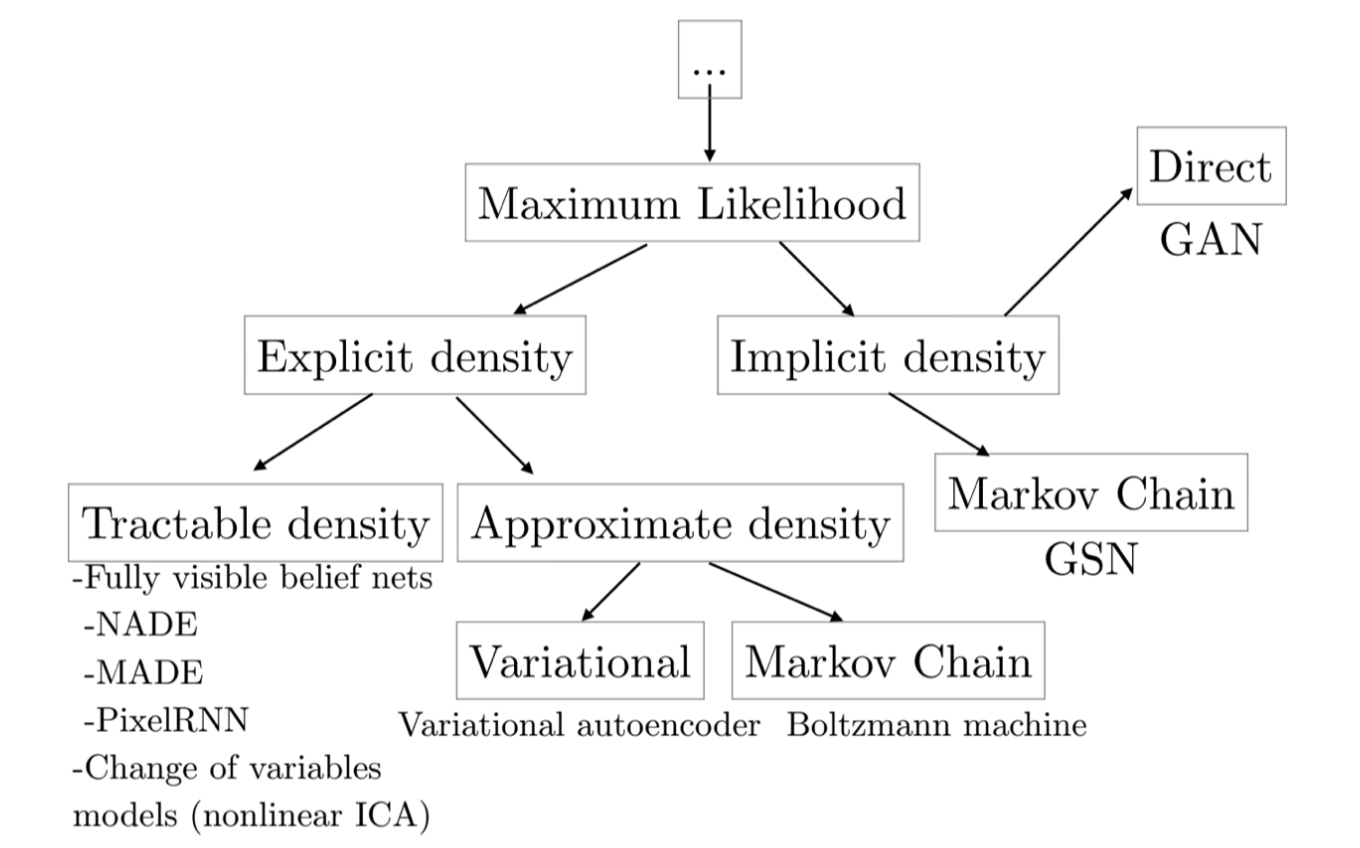
\includegraphics[width=0.45\textwidth]{figures/GAN_generative_models_overview_2.png}
		\caption{Overview of generative models}
		\label{fig:GAN_generative_models_overview}
	\end{figure}
\end{itemize}
\subsection{Generative Adversarial Networks}
\begin{itemize}
	\item Adversarial training of generator vs discriminator
	\begin{figure}[ht!]
		\centering
		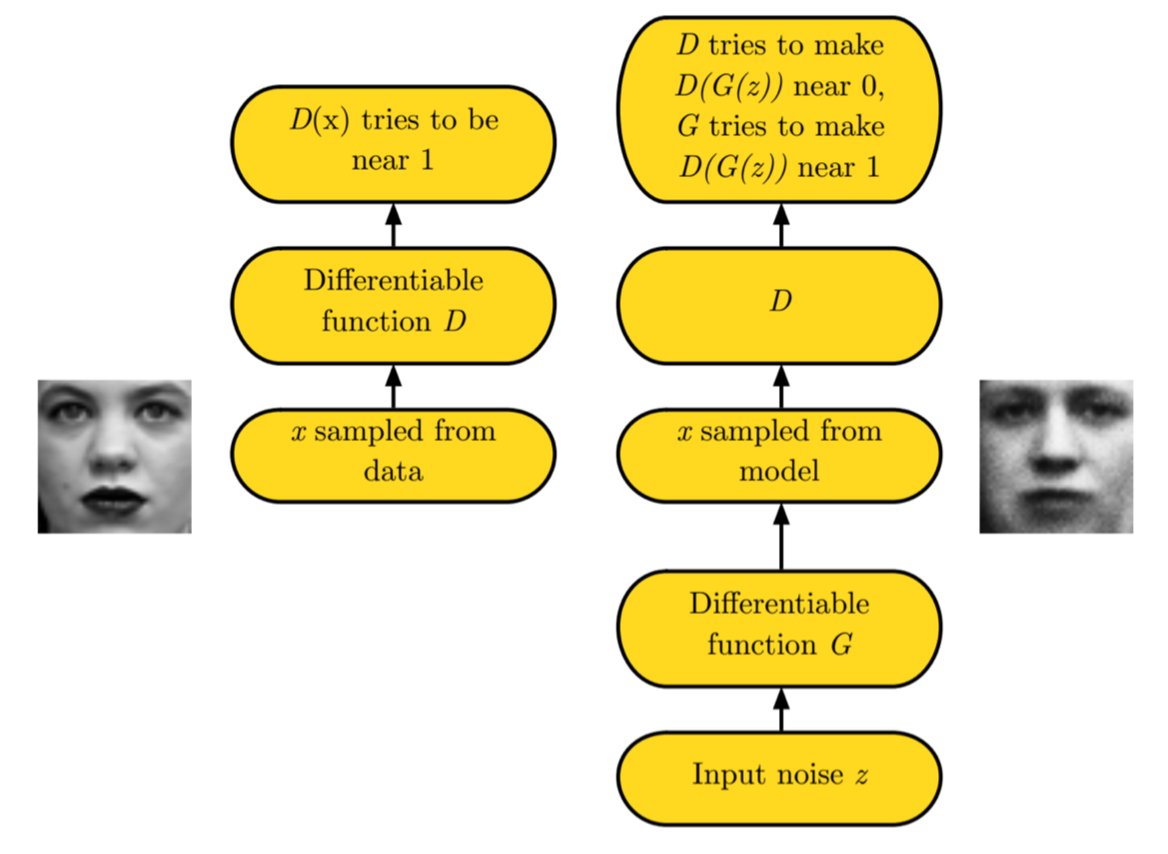
\includegraphics[width=0.45\textwidth]{figures/GAN_pipeline.png}
		\caption{Pipeline of adversarial GAN training}
		\label{fig:GAN_pipeline}
	\end{figure}
	\item The generator is a (mostly deconvolutional) network that takes noise $z$ as input, and creates fake images. The discriminator tries to distinguish between fake and real images
	\item Trained in a minimax game fashion, the loss function resembles the Jensen-Shannon divergence:
	\begin{equation*}
		\begin{split}
			\min_G \max_D V(G,D) & = \mathbb{E}_{\bm{x}\sim p_{\text{data}}(\bm{x})} \left[\log \left(D\left(\bm{x}\right)\right)\right] + \mathbb{E}_{\bm{z}\sim p_{z}(\bm{z})} \left[\log\left(1 - D\left(G\left(\bm{z}\right)\right)\right)\right] \\
			J^{(D)} & = - \frac{1}{2}\mathbb{E}_{x\sim p_{\text{data}}}\left[\log D(x)\right] - \frac{1}{2}\mathbb{E}_{z\sim p_{z}}\left[\log 1 - D(G(z))\right]\\
			J^{(G)} & = - \frac{1}{2}\mathbb{E}_{z\sim p_{z}}\left[\log D(G(z))\right]\\
		\end{split}
	\end{equation*}
	\item Loss of generator is changed from $\log 1 - D(G(z))$ because otherwise the gradients of the generator vanish for a too strong discriminator 
	\item Divergence is important and can strongly influence the behavior of model
	\begin{equation*}
		\begin{split}
			D_{KL}\left(p(x)\lVert q^{*}(x)\right) = \int p(x) \log \frac{p(x)}{q^{*}(x)} dx & \implies \text{if } p(x)>0, \text{ then } q(x)>0\\
			D_{KL}\left(q^{*}(x)\lVert p(x)\right) = \int q^{*}(x) \log \frac{q^{*}(x)}{p(x)} dx & \implies \text{if } p(x)=0, \text{ then } q(x)=0\\
		\end{split}
	\end{equation*}
\end{itemize}
\subsubsection{GAN training problems}
\begin{itemize}
	\item \textbf{Vanishing gradients} during training:
	\begin{itemize}
		\item If the discriminator is too bad, the generator does not get valid/accurate feedback and can therefore not learn properly
		\item If the discriminator is perfect, the generator has very low gradients as a small change does not influence the discriminator
		\begin{figure}[ht!]
			\centering
			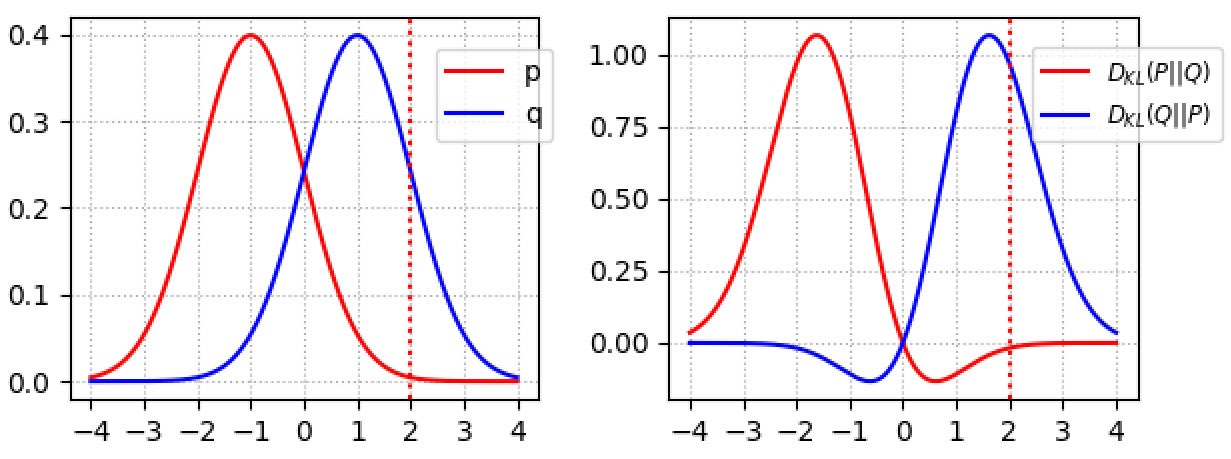
\includegraphics[width=0.4\textwidth]{figures/cv_deep_learning_GAN_vanishing_gradients.jpeg}
			\caption{Vanishing gradients problem for training with KL-divergence. When the distance between the two distributions $p$ and $q$ (respectively $P_g$ and $P_r$) is too huge, the KL divergence is very close to zero. Hence, is does not provide any strong gradients in these regions.}
		\end{figure}
	\end{itemize}
	\item \textbf{Reaching the equilibrium}
	\begin{itemize}
		\item We know that the nash equilibrium of the minimax game is $P_g=P_r$ meaning the distribution of the real data is equal to the generated data. In that case, $D$ return 0.5 no matter what example we put in (as both distributions are equal).
		\item However, it has been shown that such cost functions may not converge when using gradient descent. An example is shown in Figure~\ref{fig:GAN_reaching_equilibrium}.
		\begin{figure}[ht!]
			\centering
			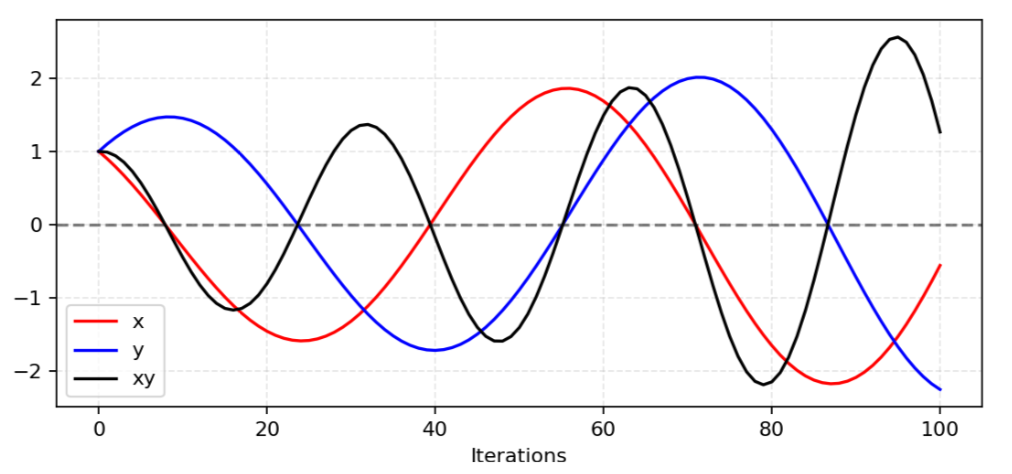
\includegraphics[width=0.4\textwidth]{figures/cv_deep_learning_GAN_oscillating.png}
			\caption{Oscillating behavior of a non-cooperative game where $\min_x \max_y V(x,y) = x\cdot y$. The equilibrium $x=y=0$ is never reached.}
			\label{fig:GAN_reaching_equilibrium}
		\end{figure}
	\end{itemize}
	\item \textbf{Mode collapse}
	\begin{itemize}
		\item A GAN suffers from a mode collapse if the generator limits its predictions/generated distribution to a few samples/modes.
		\item For example in case of the MNIST dataset, this would mean that the generator only creates numbers of one or two different digits. Although a full mode collapse is rarely the case, partial mode collapses frequently occur
		\item In order to create a mode collapse, the gradients regarding the noise $\bm{z}$ must be very low/close to zero. This can for example happen if we fix the discriminator and the generator converges to the optimal image $\bm{x}^*$ that fools the discriminator the most
		\item Once the generator collapse to one mode, the discriminator will learn that this mode is purely/mostly generated and thus changes its predictions. The generator will address that by changing the mode (note that as $\partial L/\partial \bm{z}\approx 0$, we will just collapse to the next mode and are not able to escape this loop).
		\item In the end, this turns into a cat-and-mouse game between the generator and discriminator, and will not converge (see Figure~\ref{fig:GAN_mode_collapse}).
		\begin{figure}[ht!]
			\centering
			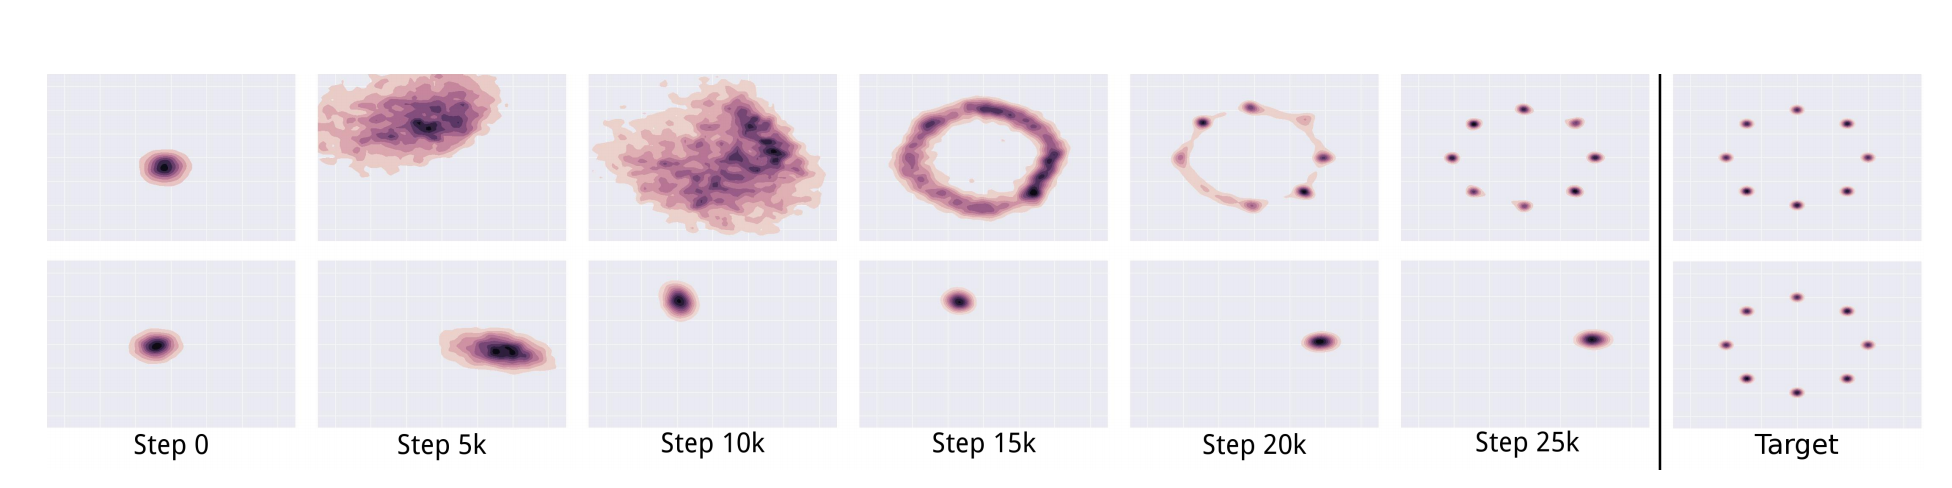
\includegraphics[width=0.6\textwidth]{figures/cv_deep_learning_GAN_mode_collapse.png}
			\caption{\textit{Top row}: optimal convergence of generator distribution to 8 modes. \textit{Bottom row}: Sample of a mode collapse after 10k iterations. The generator is only able to generate a single mode.}
			\label{fig:GAN_mode_collapse}
		\end{figure}
	\end{itemize}
	\item \textbf{Low dimensional support}
	\begin{itemize}
		\item The KL and JS divergence work best for overlapping distributions as neither of them is 0 (numerical instability)
		\item However, during training, the training distribution is not perfect, and as we have high dimensional data, both distributions are less likely to overlap much
		\item Also, it is easy for the discriminator to find a line in between them
	\end{itemize}
\end{itemize}
\subsubsection{GAN improvements}
\begin{itemize}
	\item \textbf{Wasserstein GAN}
	\begin{itemize}
		\item Instead of KL/JS, use Wasserstein (Earth Mover's) Distance:
		$$\mathcal{W}(p_r, p_g) = \inf\limits_{\gamma \sim \prod (p_r,p_g)} \mathbb{E}_{(x,y)\sim \gamma}|x-y|$$
		\item Intuitive explanation: how much do I have to move from one distribution to get the other one. Thus, the distance is even meaningful for non-overlapping distributions
	\end{itemize}
	\item \textbf{Usage of labels}
	\begin{itemize}
		\item Learning a conditional model $p(y|x)$ often generates better samples than from a random distribution
		\item One example are conditional GANs where we have given a ground truth
	\end{itemize}
	\item \textbf{Label smoothing}
	\begin{itemize}
		\item Train the discriminator to predict $D(x)\approx 1 - \alpha$ instead of 1
		\item Has been shown to be a good regularization by preventing the discriminator to be overconfident
		\item In addition, the gradients of the generator do less likely explode
	\end{itemize}
	\item \textbf{Virtual batch normalization}
	\begin{itemize}
		\item Batch Normalization can significantly help in neural networks
		\item However, in GANs, it leads to high intra-batch correlation
		\item Solution: \textit{virtual batch normalization} where we select a reference batch which is fixed during training, and combine it with the statistics of the current batch. Reduces overfitting on reference batch and intra-batch correlation
	\end{itemize}
\end{itemize}
\subsubsection{GAN open questions}
\begin{itemize}
	\item \textbf{Mode collapse}: How to prevent a model to suffer from mode collapse. One idea is penalizing the model is features are too similar, or allowing discriminator to see across batch elements. But these solutions are more heuristic tries and no theoretical solution
	\item \textbf{Evaluation of GANs}: GANs are currently judged by their qualitative results/predictions, but there is no quantitative measurement yet
	\item \textbf{Discrete outputs}: The generator and discriminator need to be differentiable, and thus discrete outputs are not possible. There are some workarounds, but no real theoretically sound solution.
	\item \textbf{Semi-supervised classification}: How to combine a GAN training and discriminative model efficiently (discriminator predicts class and fake/real at the same time)
\end{itemize}
\subsection{Boltzmann machines}
\begin{itemize}
	\item A Boltzmann distribution is defined by $p(x) = \frac{1}{Z}\exp\left(-E\left(x\right)\right)$ where $E(x)$ is a energy function described by our model, and $Z=\sum\limits_x \exp\left(E\left(x\right)\right)$ a normalization constant
	\item The benefit of defining a distribution like that is that our model can use any output values between $[-\infty, \infty]$ instead of being constrained to $[0,1]$
	\item A problem is that even if $x$ is binary, the normalizing constant $Z$ gets out of hands (sum over $2^{n}$ combinations for $n$ dimensional $x$). Thus, we limit the computations by only considering pairwise relations
	\item Pairwise relations modeled by $E(x)=-x^TWx-b^Tx$. Learning $W$ and $b$ by maximizing the likelihood of the data
	\item Problem: $W$ is still of size $n^2$ which can be too large for e.g. images ($256\times 256$ leads to $4.2$ billion parameters in $W$) $\Rightarrow$ Restricted Boltzmann machines
\end{itemize}
\subsubsection{Restricted Boltzmann machines}
\begin{itemize}
	\item Restrict model by additional bottleneck over $h$ latents
	$$E(x,h) = -x^T W h - b^T x - c^T h, \hspace{2mm} p(x) = \frac{1}{Z}\sum_h \exp\left(-E\left(x,h\right)\right)$$
	\item This function is not in the form of a energy function anymore (because of the sum). We can rewrite it as:
	\begin{equation*}
		\begin{split}
			F(x) & = -b^T x - \sum_i \log \sum_{h_i} \exp\left(h_i\left(c_i + W_i x\right)\right)\\
			p(x) & = \frac{1}{Z} \exp\left(-F(x)\right)\\
			Z & = \sum\limits_x \exp\left(-F(x)\right)
		\end{split}
	\end{equation*}
	\item Can be represented as a single MLP layer (undirected) with less hidden units
	\item Compared to simple Boltzmann machine, we can express higher-order relations 
	\item Every hidden unit is independent of each other, and the same for input $x$:
	$$p(h|x) = \prod_j p(h_j|x, \theta), \hspace{2mm} p(x|h) = \prod_i p(x_i|h, \theta) $$
	\item We can now reformulate the conditional probabilities as sigmoids \textbf{iff} $h$ and $x$ are still binary:
	$$p(h_j|x, \theta) = \sigma\left(W_{:,j} x + b_j\right), \hspace{2mm}p(x_i|h, \theta) = \sigma\left(W_{i,:} h + c_i\right)$$
	\item The loss is maximizing the log likelihood:
	$$\mathcal{L}(\theta) = \frac{1}{N}\sum_n \log p(x_n|\theta) = \frac{1}{N}\sum_n\left[- F(x) - \log Z\right]$$
	\item The gradients can be computed accordingly:
	\begin{equation*}
		\begin{split}
			\pd{\log p(x_n|\theta)}{\theta} & = -\sum_h p(h|x_n, \theta) \pd{E(x_n,h| \theta)}{\theta} + \sum_{\tilde{x}, h} p(\tilde{x}, h|\theta) \pd{E(\tilde{x}, h|\theta)}{\theta}\\
		\end{split}
	\end{equation*}
	Problem: second term is sum over $x$ and $h$ $\Rightarrow$ high-dimensional, hard to compute
	\item One way to do it is using contrastive divergence: sample $h_0 \sim p(h|x)$, and $x_1 \sim p(x|h_0)$, etc. In practice, a single sample is mostly sufficient
	\item \textbf{Deep Belief Network}: RBM are still models of single layer, we can also use a stack of RBMs. First layer is directed, others not. Our joint pdf is $p(x, h_1, h_2) = p(x|h_1)\cdot p(h_1|h_2)$
	\item \textbf{Deep Boltzmann machines}: also a stack of RBMs, but with undirected first layer
	\begin{itemize}
		\item Hence, we get $p(h_2^{k}|h_1, h_3) = \sigma \left(W_1^{:,k}h_1 + W_3^{k,:}h_3 \right)$
		\item Computing gradients is intractable $\Rightarrow$ approximate by sampling
	\end{itemize}
\end{itemize}
\subsection{Variational Autoencoders}
\begin{itemize}
	\item We assume an underlying, lower-dimensional data distribution $p(z)$ with which we can model our data distribution $p(x,z)=p(x|z)p(z)$
	\item Therefore, we need to model $p(z|x)$ which is often not easy to compute. In variational inference, we approximate the true posterior by $q_{\varphi}(z)$ (approximated posterior does not have to depend on observed $x$, e.g. in VAE it does)
	\item Our goal is to maximize $p(x)$. As this is intractable, we use the ELBO:
	\begin{equation*}
		\begin{split}
			\log p(x) & = \log \int p(x,z)dz \\
			& = \log \int q_{\varphi}(z) \frac{\int p(x,z)}{q_{\phi}(z)} dz\\
			& = \log \mathbb{E}_{q_{\varphi}(z)}\left[\frac{p(x,z)}{q_{\varphi}(z)}\right]\\
			& \geq \mathbb{E}_{q_{\varphi}(z)}\left[\log \frac{p(x,z)}{q_{\varphi}(z)}\right]\\
			& = \mathbb{E}_{q_{\varphi}(z)}\left[\log p(x|z)\right] - \text{KL}\left(q_{\varphi}(z)||p(z)\right) = \text{ELBO}_{\theta, \varphi}\left(x\right)
		\end{split}
	\end{equation*}
	\item The distance between $\log p(x)$ and the ELBO is the KL divergence to the true (unknown) posterior:
	$$\log p(x) - \text{KL}\left(q_{\varphi}(z)||p(z|x)\right) = \mathbb{E}_{q_{\varphi}(z)}\left[\log p(x|z)\right] - \text{KL}\left(q_{\varphi}(z)||p(z)\right)$$
	\item Thus, maximizing the ELBO either increases the log likelihood or optimizes the approximated posterior
	\item Variational Autoencoders make $q_{\varphi}(z)$ dependent of $x$, and model $p_{\theta}(x|z)$ as well:
	$$\text{ELBO}_{\theta, \varphi}\left(x\right) = \mathbb{E}_{q_{\varphi}(z|x)}\left[\log p_{\theta}(x|z)\right] - \text{KL}\left(q_{\varphi}(z|x)||p_{\lambda}(z)\right)$$
	Note that $p_{\lambda}(z)$ is not optimized, and its parameters $\lambda$ just describe the prior (e.g. standard Gaussian) 
	\item The loss function for a VAE is the negative ELBO, where we approximate the expectation by a single sample. The KL is mostly chosen to be analytically solvable (e.g. for two Gaussian) to prevent a Monte-Carlo approximation of the integral 
	\item However, we face a problem when we try to compute the gradients for $\nabla_{\varphi} \mathcal{L}$. Using Monte-Carlo integration has high variance, and sampling is non-continuous operation
	\item \textbf{Reparameterization trick}: sample from external, constant distribution, and transform this sample into a sample of the modeled distribution. For Gaussian: $z = \mu_q + \sigma_q \cdot \epsilon$
\end{itemize}
\subsubsection{Improvements of VAE}
\begin{itemize}
	\item \textbf{Encoder distribution}
	\begin{itemize}
		\item Modeling $q(z|x)$ as Gaussian makes training and implementation easy, but assumes that true posterior is also Gaussian, or can be at least approximated by one
		\item Simple option: use different task-specific distribution like e.g. hyperspherical, however not always suitable
		\item We can improve the complexity of this posterior by plugging in a Normalizing flow on top of the encoder output
		\begin{equation*}
		\begin{split}
		z_0 \sim q_0(z|x) & = \mathcal{N}(z|\mu(x), \text{diag}(\sigma^2(x)))\\
		q_K(z|x) & = q_0(z|x) \cdot \left|\text{det}\pd{f_K(z_{k-1})}{z_{k-1}}\right|\\
		\end{split}
		\end{equation*}
		\item The ELBO is added with an additional term during training
		$$\text{ELBO} = \mathbb{E}_{q_{\varphi}(z|x)}\left[\log p_{\theta}(x|z)\right] - \text{KL}\left(q_{\varphi}(z|x)||p_{\lambda}(z)\right) + \mathbb{E}_{z_0 \sim q_0(z_0|x)}\left[\sum_{k=1}^{K} \log \left|\text{det}\pd{f_k(z_{k-1})}{z_{k-1}}\right|\right]$$
	\end{itemize}
	\item \textbf{Prior optimization}
	\begin{itemize}
		\item We assume a prior $p(z)$ which is for example Gaussian, but cannot make sure that every point of the prior actually has a realistic counterpart in the original $x$ space
		\item The optimal prior is the averaged distribution over all data samples: $q^{*}(z) = \frac{1}{N}\sum_{n=1}^{N} q_{\varphi}(z|x_n)$
		\item However, summing over all data point is infeasible. Thus, approximate it by $K$ pseudo-inputs $u_k$ that are trained via standard SGD in the framework:
		$$p_\lambda(z) = \frac{1}{K} \sum_{k=1}^{K} q_{\varphi}(z|u_k)$$
	\end{itemize}
	
\end{itemize}
\subsection{Normalizing flows}
\begin{itemize}
	\item VAE cannot model $p(x)$ directly because of the intractable formulation ($p(x) = \int p(x,z)dz$)
	\item Normalizing Flows solve that problem by using a series of invertible transformation that allow more complex latent distributions than Gaussian
	\item The models can therefore be trained on directly maximizing the log likelihood instead of using the ELBO or similar
	\item A normalizing flow consists of multiple flows that transform a simple Gaussian distribution step by step in the data distribution (see Figure~\ref{fig:NF_concept})
	\item Every flow shifts the probability mass specified by parameters (determined by e.g. a NN, see Figure~\ref{fig:NF_density_shift})
	\begin{figure}[ht!]
		% NF_density_shift.png
		\centering
		\begin{subfigure}{0.7\textwidth}
			\centering
			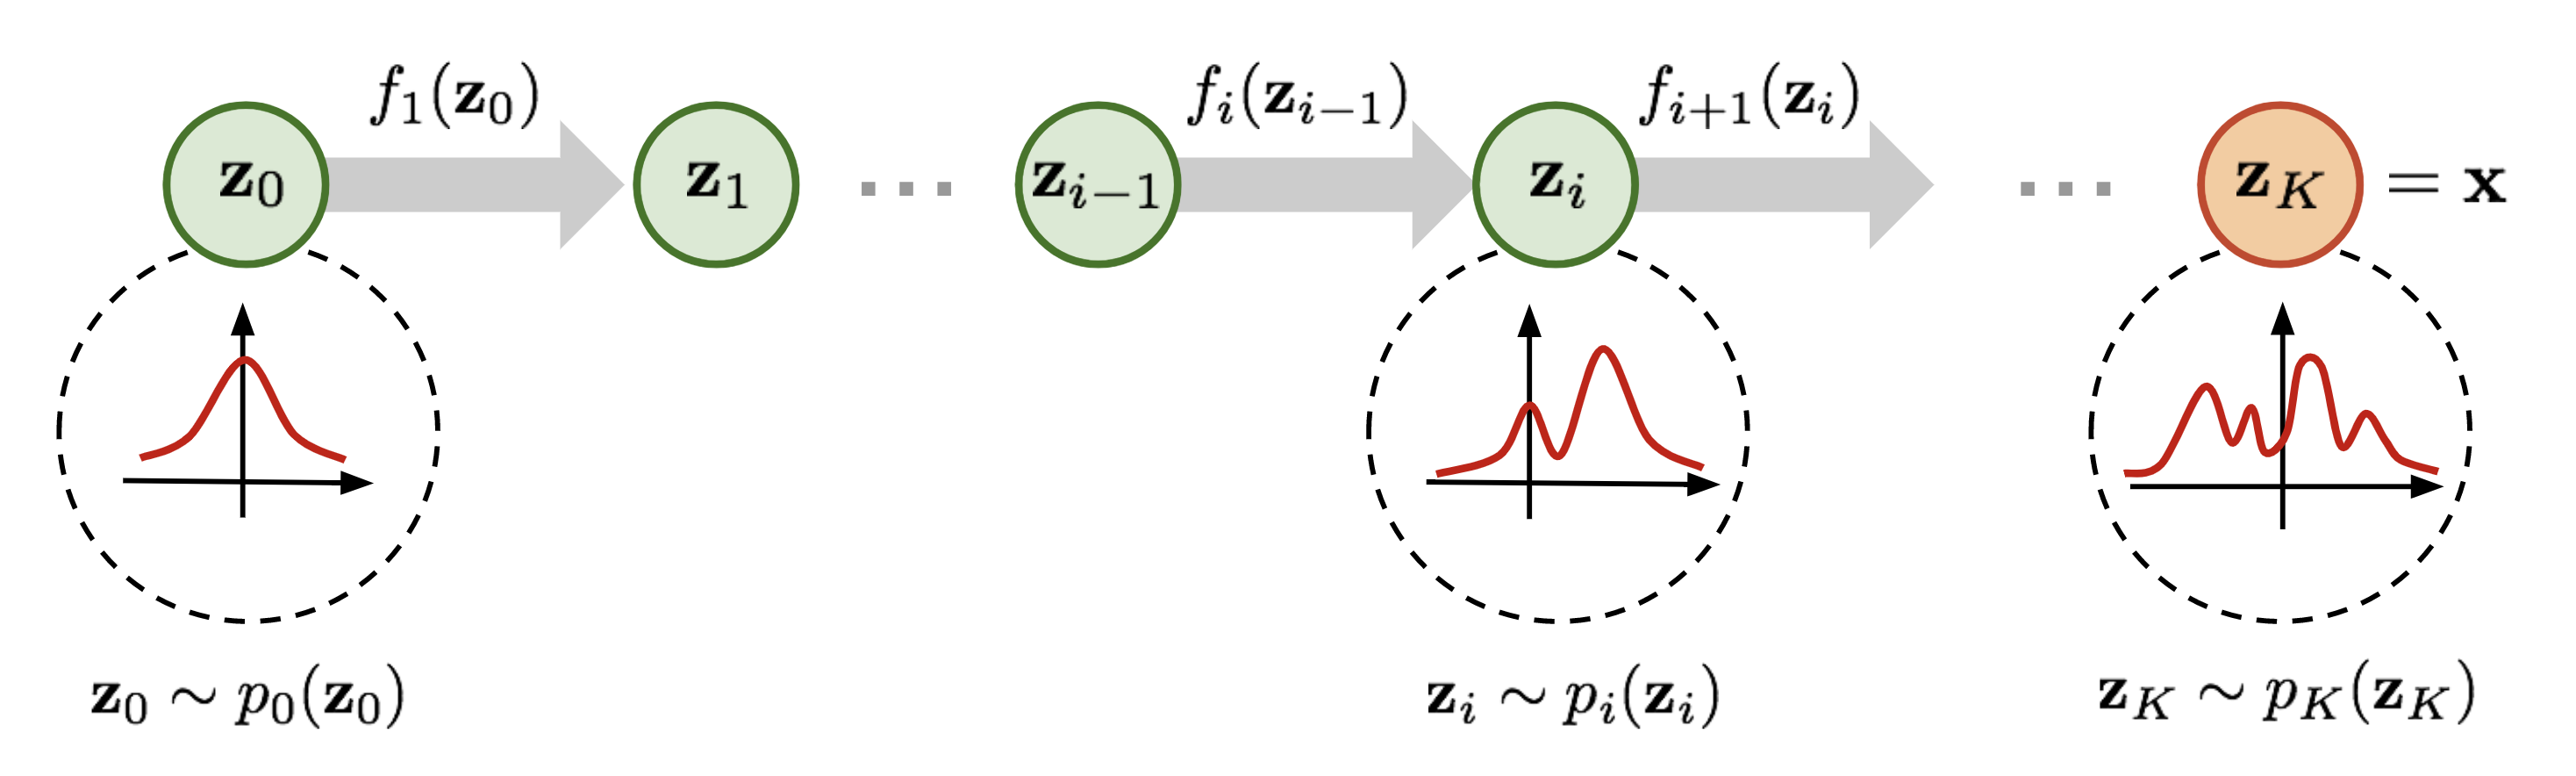
\includegraphics[width=\textwidth]{figures/NF_concept.png}
			\caption{General concept of stacking multiple flows}
			\label{fig:NF_concept}
		\end{subfigure}
		\hspace{8mm}
		\begin{subfigure}{0.2\textwidth}
			\centering
			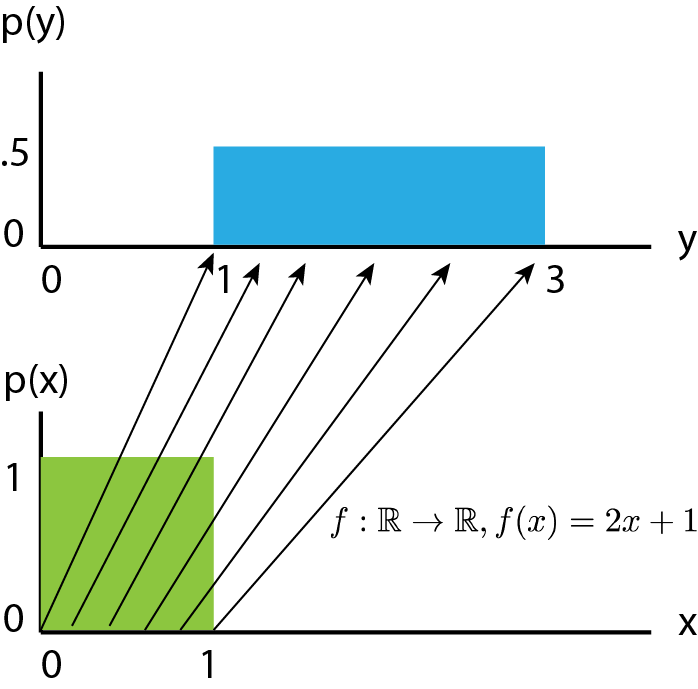
\includegraphics[width=\textwidth]{figures/NF_density_shift.png}
			\caption{Shifting density}
			\label{fig:NF_density_shift}
		\end{subfigure}
		\caption{Outline of how a normalizing flow works}
		\label{fig:NF}
	\end{figure} 
	\item Mathematically, we can define a normalizing flow by:
	\begin{equation*}
		\begin{split}
			x & = z_k = f_k \circ f_{k-1} \circ ... \circ f_1 (z_0) \to z_i = f_i(z_{i-1})\\
			p(z_i) & = p(z_{i-1}) \cdot \left|\det \frac{f_{i}^{-1}}{z_i}\right| \implies p(x) = p(z_0) \cdot \prod_{i=1}^{K} \left|\det \frac{f_{i}^{-1}}{z_i}\right|\\
			\log p(x) & = \log p(z_0) - \sum_{i=1}^{K} \log \left|\det \frac{f_{i}}{z_i}\right|
		\end{split}
	\end{equation*}
	\item Requirements: $f$ must be invertible (dimensions of $x$ and $z$ equal), and the Jacobian must be easy to compute (i.e. triangular)
\end{itemize}
\section{Bayesian Deep Learning}
\begin{itemize}
	\item Bayesian machine learning: holding a distribution per latent variable instead of single value
	\item Benefits of Bayesian
	\begin{itemize}
		\item Ensemble modeling (better accuracies)
		\item Uncertainty estimates, preventing overconfident networks
		\item Model compression (have prior that pushes weights towards 0)
		\item \TODO{Think of more}
	\end{itemize}
\end{itemize}
\subsection{Epistemic uncertainty}
\begin{itemize}
	\item \textit{Epistemic uncertainty}: dataset limits
	\item Uncertainty that is introduced by dataset limits (unseen data $\Rightarrow$ how certain are the weights)
	\item Can be reduced by increasing the amount of data
	\item Important for safety-critical applications and small datasets
	\item Hard to model because posterior is usually intractable for complex functions like NN
	$$p(w|x,y) = \frac{p(x,y|w)p(w)}{\int p(x,y|w)p(w)dw}$$
	\item \textbf{Monte-Carlo Dropout}: apply dropout during testing (Bernoulli-distribution over weights as variational distribution). The variance/uncertainty derived from there approximates uncertainty gained by variational framework. 
	\begin{itemize}
		\item \textit{Advantages}: every standard NN can be turned into a Bayesian NN. Very easy to train and no inference network necessary
		\item \textit{Drawbacks}: expensive, have to rerun model several times on data. Not very accurate (depends on activation function etc.)
	\end{itemize}
	\item \textbf{Deep Gaussian Process}: predict mean and variance for every data point.
	\begin{itemize}
		\item The predictive distribution is $p(y|x,X,Y) = \int p(y|x,w)p(w|X,Y)dw$
		\item The likelihood term is a Gaussian $p(y|x,w)=\mathcal{N}(y; \hat{y}(x,w), \tau^{-1}I_D)$ where $\hat{y}(x,w)$ is a NN and $\tau^{-1}$ the model precision that can be derived from MC dropout
		\item For the posterior, we use variational approximation: $p(w|X,Y)\approx q(w)$. In case of MC dropout, we have $\tilde{W}_i = W_i\cdot \text{diag}\left(\left[z_{i,j}\right]_{1}^{K_i}\right), z_{i,j}\sim \text{Bernoulli}\left(p_i\right)$ where $\tilde{W}_i$ are the weights with applied dropout
		\item Minimize loss $\mathcal{L}= - \int q(w)\log p(Y|X,w)dw + KL\left(q(w)||p(w|X,Y)\right)$. First term is approximated by Monte-Carlo integration (equivalent to sampling dropout), and second can be approximated analytically
	\end{itemize}
	\item Over-paramterized models give better uncertainty estimates as they capture bigger class of models. However, they also need higher dropout rates
\end{itemize}
\subsection{Aleatoric uncertainty}
\begin{itemize}
	\item \textit{Aleatoric uncertainty}: data uncertainty
	\item Uncertainty due to the nature of data (noise/hard to predict accurate. Example: depth estimation with bad sensor)
	\item Can be reduced by better data (better sensors, multiple different sensors, etc.)
	\item \textit{Data-dependent/heteroscedastic aleatoric uncertainty}: specific raw inputs like images that are hard to interpret
	\begin{itemize}
		\item Can be modeled by predicting a variance term per data point to reduce loss
		$$\mathcal{L} = \frac{\lVert y_i - \hat{y}_i\rVert^2}{2\sigma_i^2} + \log \sigma_i$$
		If variance low, the loss is weighted higher, but the $\log$ term is smaller $\Rightarrow$ trade-off
	\end{itemize}
	\item \textit{Task-dependent/homoscedastic aleatoric uncertainty}: introduced by task like semantic segmentation or depth estimation (hard at edges). Possible solution: train on multiple tasks like edge detection
	\begin{itemize}
		\item We can as well introduce a variance term, but shared by all data points (task individual):
		$$\mathcal{L} = \frac{\lVert y_i - \hat{y}_i\rVert^2}{2\sigma^2} + \log \sigma$$
	\end{itemize}
\end{itemize}
\subsection{Bayes by Backprop}
\begin{itemize}
	\item Start from a NN with a distribution over its weights
	\item Train weights to approximate the true posterior well (similar to ELBO just with $p(\mathcal{D})=1 \Rightarrow \log p(\mathcal{D}) = 0$)
	$$\text{KL}\left(q\left(w|\theta\right)||p\left(w|\mathcal{D}\right)\right) = \text{KL}\left(q\left(w|\theta\right)||p\left(w\right)\right) - \int q(w|\theta) \log p(\mathcal{D}|w)dw$$
	First term pushes distributions towards prior, and second towards modeling the data well
	\item Compute by Monte-Carlo integration (over distribution $q(w|\theta)$) for \textit{both} terms:
	$$\mathcal{L} = \log q(w_s|\theta) - \log p(w_s) - \log p(\mathcal{D}|w_s) \hspace{2mm}\text{ where }\hspace{2mm} w_s\sim q(w_s|\theta)$$
	\item Example: assume a Gaussian variational posterior on the weights $w=\mu + \epsilon \cdot \log(1 + \exp\rho))$ (standard deviation with softplus trick for always positive values). Learn parameters $\mu$ and $\rho$ per weight
	\begin{figure}[ht!]
		\centering
		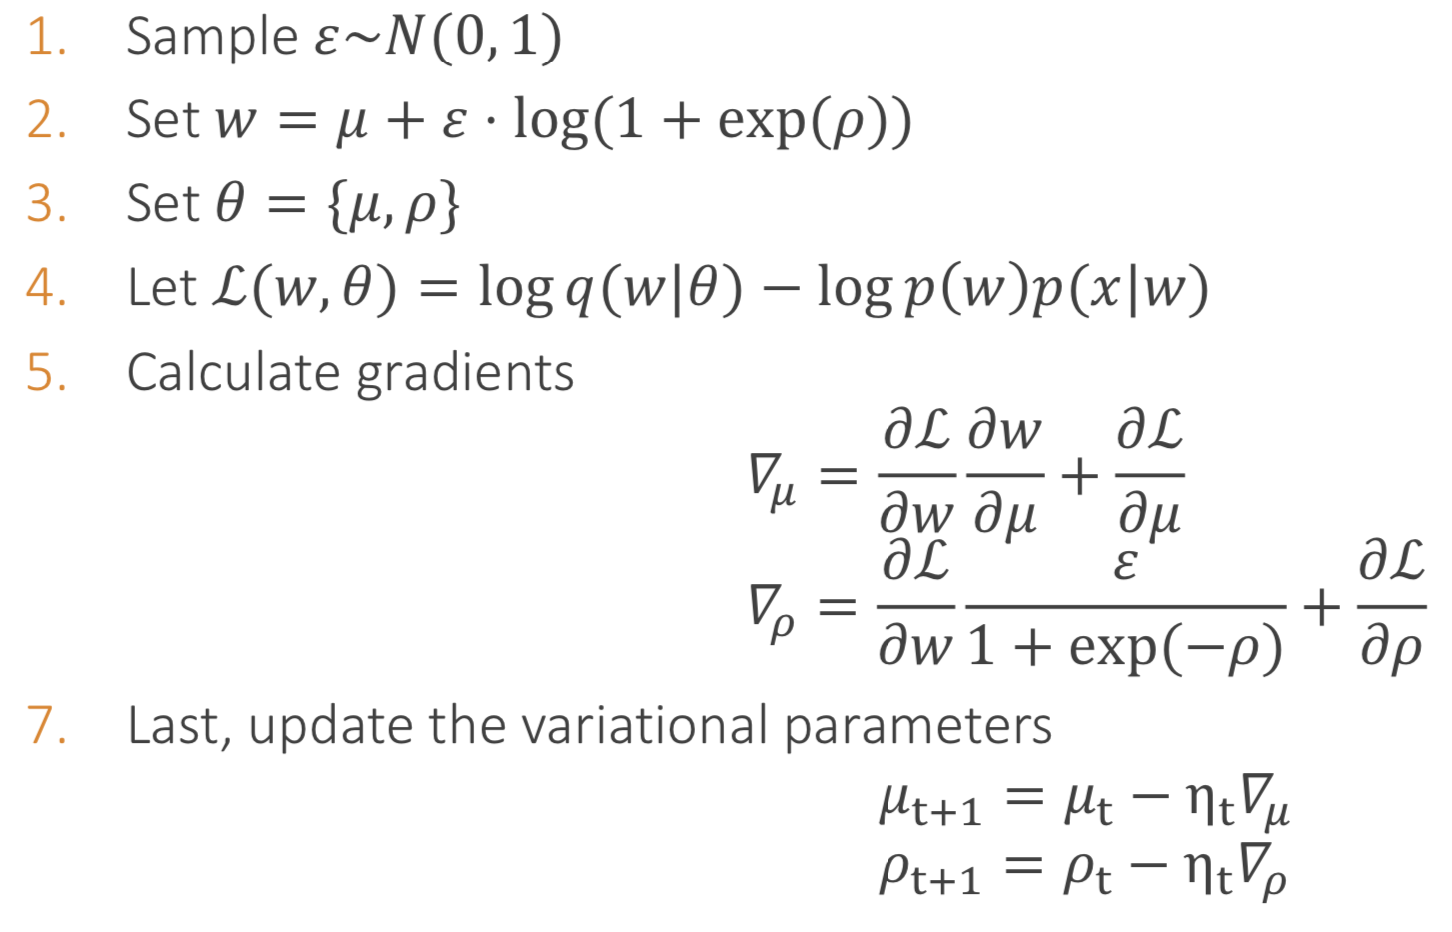
\includegraphics[width=0.4\textwidth]{figures/Bayes_By_Backprop.png}
	\end{figure}
	\item In experiments, Bayesian NNs perform similar to plain NNs with dropout
\end{itemize}
\section{Deep Sequential Models}
\subsection{Autoregressive Models}
\begin{itemize}
	\item Generative models without latent variables, but assuming an order in the data (if there is no, create an artificial order like image from left to right, top to bottom). The likelihood is the product of conditionals:
	$$p(x)=\prod_{k=1}^{D} p(x_k|x_{j<k})$$
	\item In contrast to RNNs, there is no/not necessarily parameter sharing, and the chain cannot be of infinite length because of that
	\item \textit{Advantages}: $p(x)$ is tractable
	\item \textit{Drawbacks}: training and generation is slow due to being sequential and not parallel
\end{itemize}
\subsubsection{NADE}
\begin{itemize}
	\item Originally defined for binary inputs/data. Can be generalized for other spaces as well
	\item Every output $x_d$ is modeled by a single layer that takes as input all previous data points, and generates based on that it's prediction:
	\begin{equation*}
		\begin{split}
			p(x_d=1|x_{<d}) & = \sigma\left(V_{d,:}\cdot h_d + b_d\right), h_d = \sigma\left(W_{:,<d}\cdot x_{<d} + c\right)
		\end{split}
	\end{equation*}
	where $V\in \mathbb{R}^{D\times H}, W\in \mathbb{R}^{H\times D}, b\in \mathbb{R}^{D}, c\in \mathbb{R}^{H}$ ($H$ hidden dimensionality, $D$ input dimensions)
	\item Objective is minimizing log likelihood: $\mathcal{L} = - \log p(x) = - \sum_{k=1}^{D} p(x_k|x_{<k})$
	\begin{figure}[ht!]
		\centering
		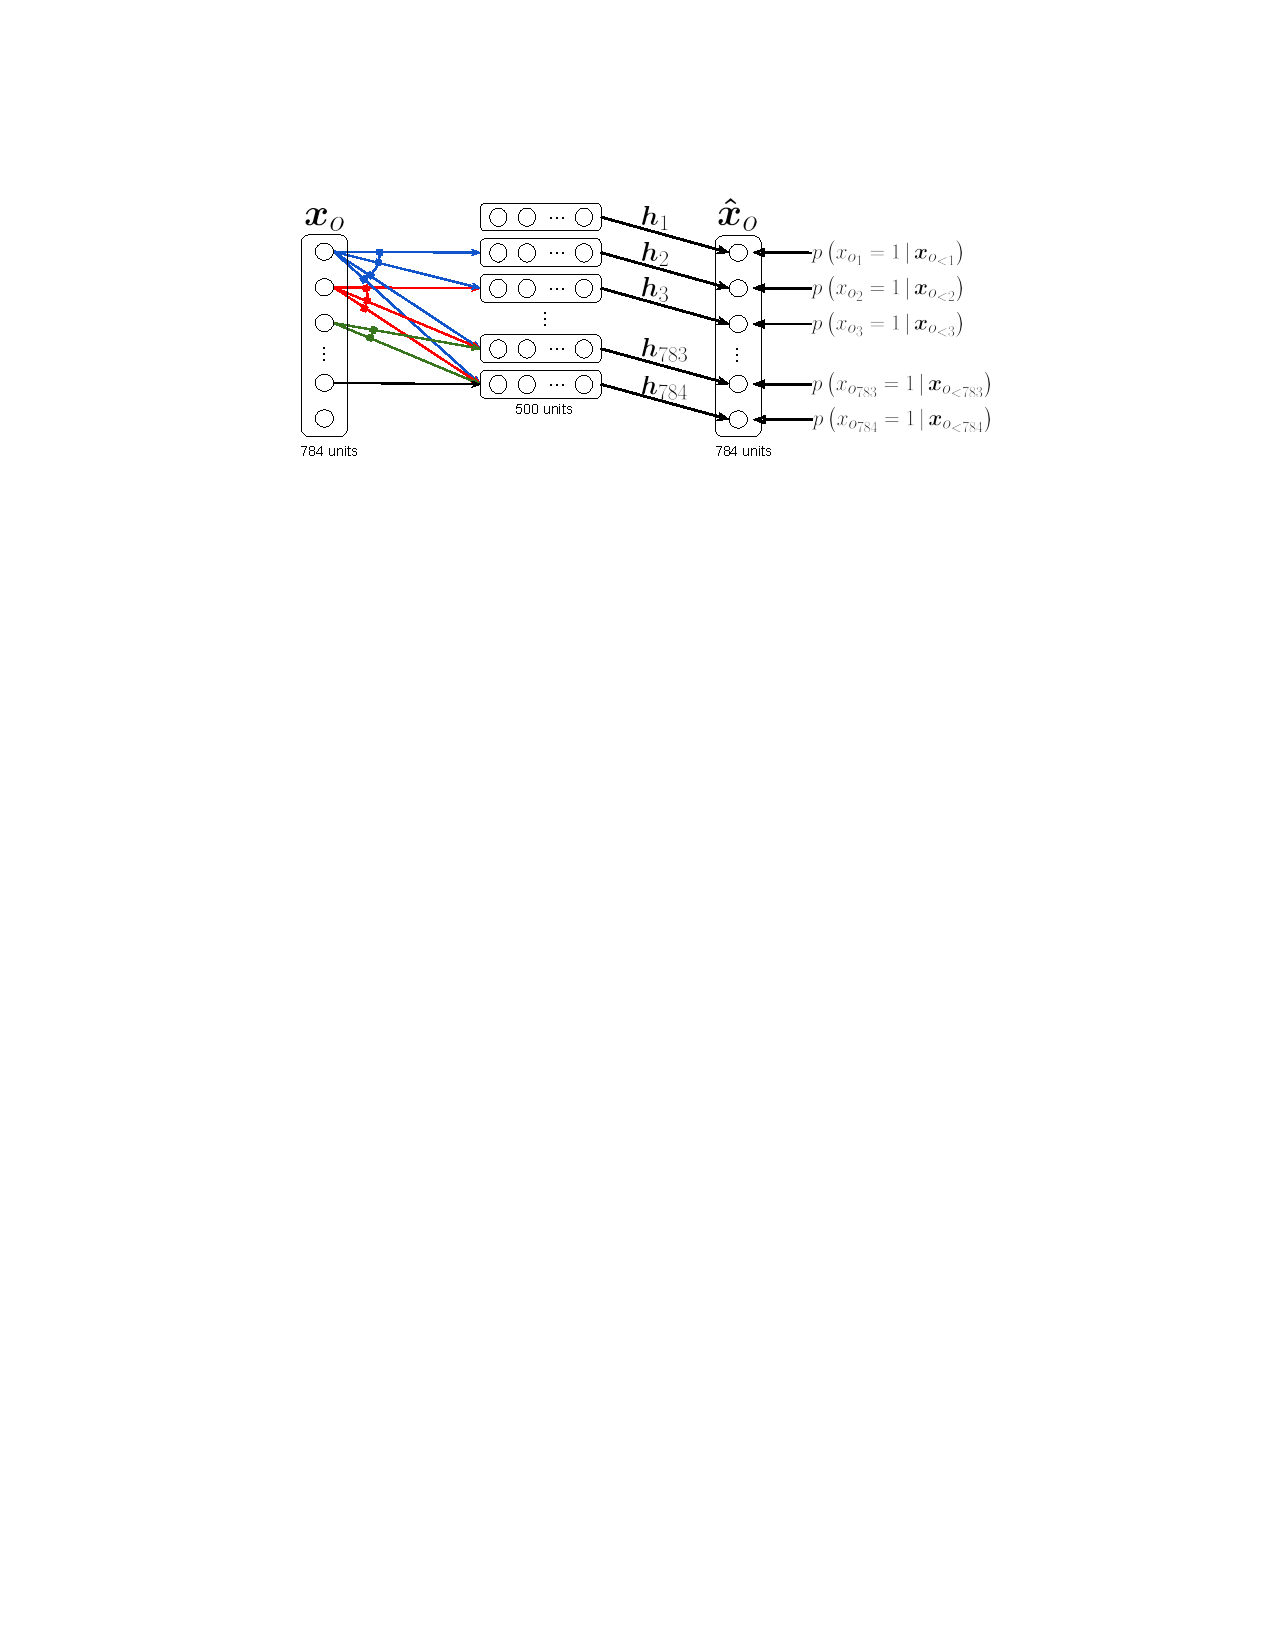
\includegraphics[width=0.6\textwidth]{figures/Autoregressive_NADE.pdf}
		\caption{Concept of NADE.}
	\end{figure}
	\item \textit{Teacher forcing}: During training, use ground truth as input for all levels. For testing, use generated samples as input (sequentially)
\end{itemize}
\subsubsection{MADE}
\begin{itemize}
	\item Use an autoencoder where we carefully mask out connections so that the output $y_d$ only depends on inputs $x_{<d}$
	\item Name ``autoencoder'' is only because we try to reproduce the input. However, note that we neither have a bottleneck nor we try to get sparsity. We just remove connections to make the outputs depending on certain inputs
	\begin{figure}[ht!]
		\centering
		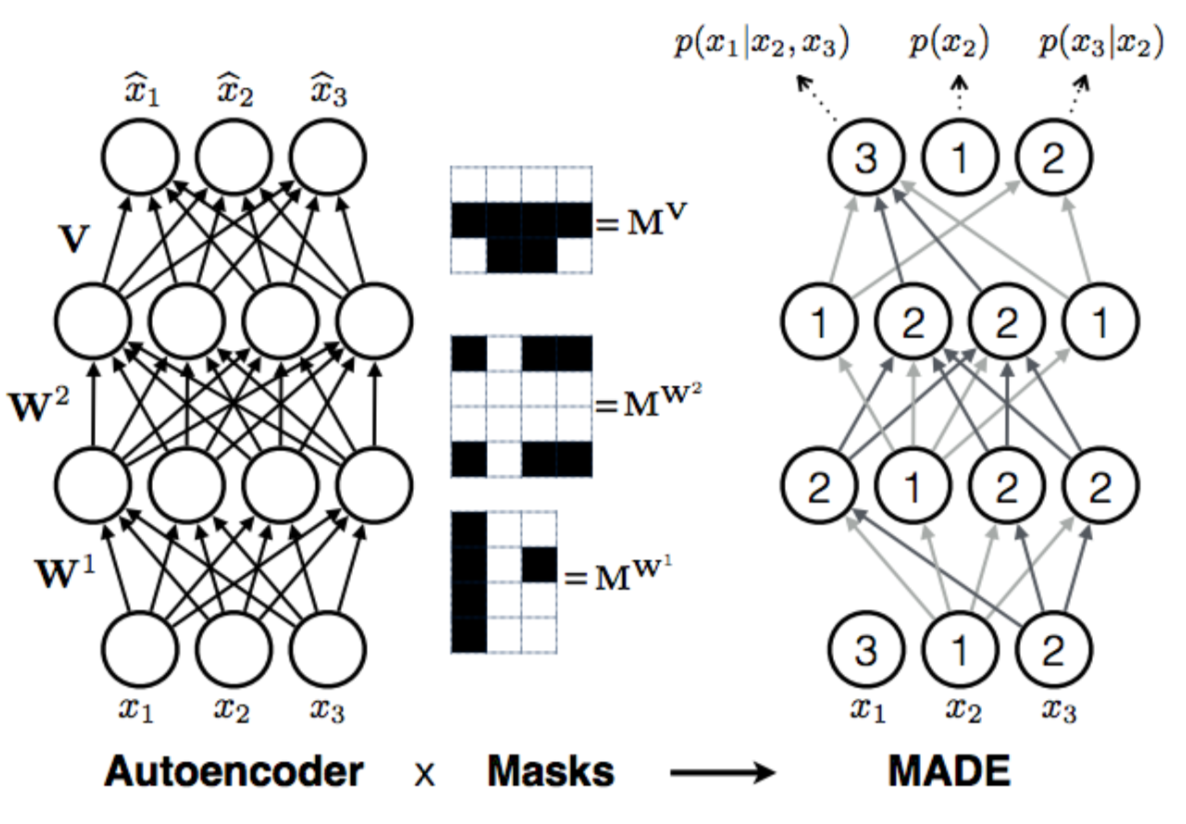
\includegraphics[width=0.4\textwidth]{figures/Autoregressive_MADE.png}
		\caption{Masked autoencoder for autoregressive models. We set certain weights to 0 (i.e. remove connections between neurons) so that the generation of $x_1$ only depends on $x_2$ and $x_3$, but not on $x_1$ itself (which would be cheating and prevent the model of being generative).}
	\end{figure}
\end{itemize}
\subsubsection{PixelRNN}
\begin{itemize}
	\item Assume row-wise pixel and sequential color generation (first red channel, then green, afterwards blue):
	$$p(x_i|x_{<i}) = p(x_{i,R}|x_{<i})\cdot p(x_{i,G}|x_{i,R}, x_{<i})\cdot p(x_{i,B}|x_{i,R}, x_{i,G}, x_{<i})$$
	\item Different ways of modeling it. LSTM variants mostly have 12 layers
	\begin{itemize}
		\item \textit{Row LSTM}: to compute next output (i.e. next hidden state), we take into consideration the three hidden states of the row above a certain pixel as ``last hidden state''. We get therefore a tri-angular shape of context. However, it thereby misses context from the row itself, and further away context. As it does not use pixels in the same row, the computation can be parallelized for a row. 
		\item \textit{Diagonal Bi-LSTM}: Uses all pixels that were generated before by using a Bi-LSTM. 
	\end{itemize}
	\begin{figure}[ht!]
		\centering
		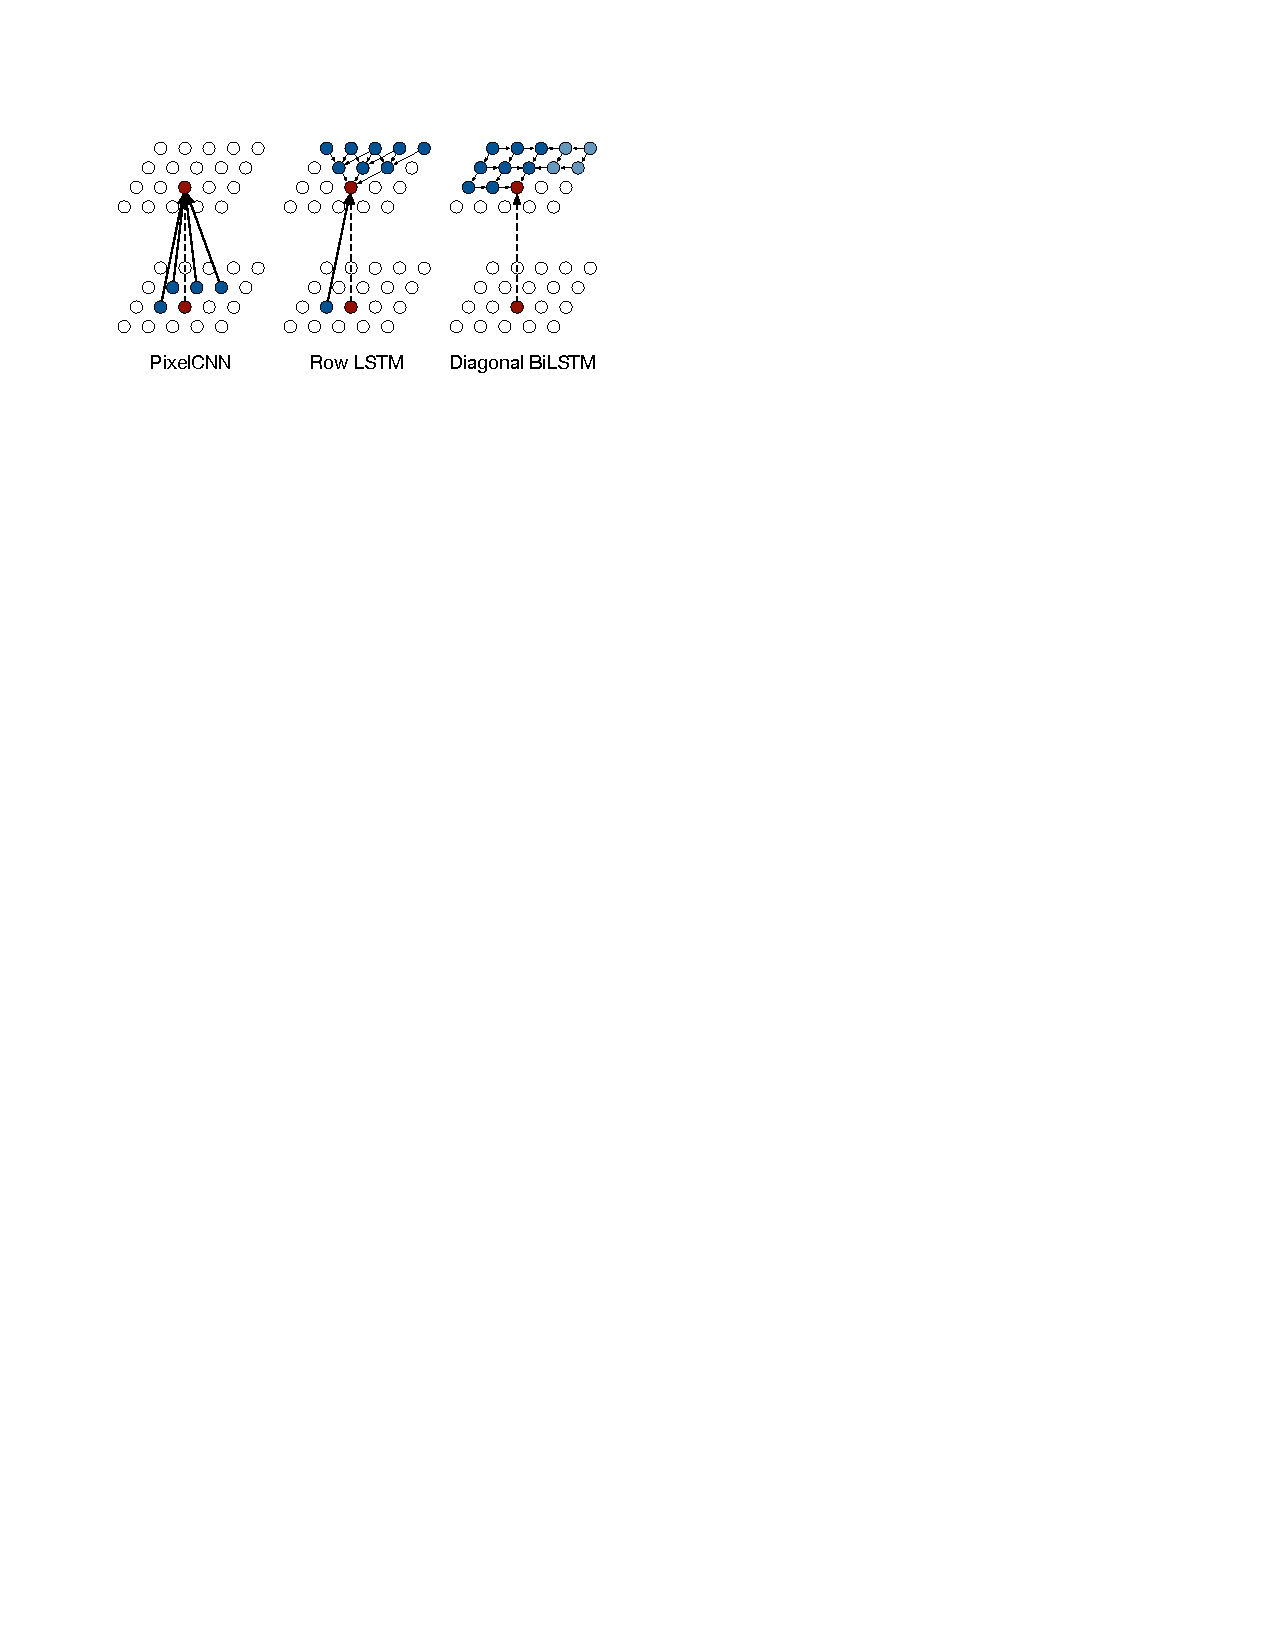
\includegraphics[width=0.4\textwidth]{figures/Autoregressive_PixelRNN.pdf}
		\caption{Comparing different methods of PixelRNN and PixelCNN. The lower level is the previous layer, and the top is the next layer. If we have a single layer PixelRNN/CNN, the lower one would be the input and the upper the generated output.}
		\label{fig:Autoregressive_PixelRNN}
	\end{figure}
	\item The architecture includes residual connections to speed up training
	\item \textit{Benefits}: good modeling of $p(x)$, reasonable image quality
	\item \textit{Disadvantages}: slow training and slow generation
\end{itemize}
\subsubsection{PixelCNN}
\begin{itemize}
	\item Replace recurrence by convolutions to speed up (at least) training
	\item Convolutions are masked so that only context from before (i.e. left and top) can be used. See Figure~\ref{fig:Autoregressive_PixelRNN} left and Figure~\ref{fig:Autoregressive_PixelCNN} for an example
	\begin{figure}[ht!]
		\centering
		\begin{subfigure}{0.3\textwidth}
			\centering
			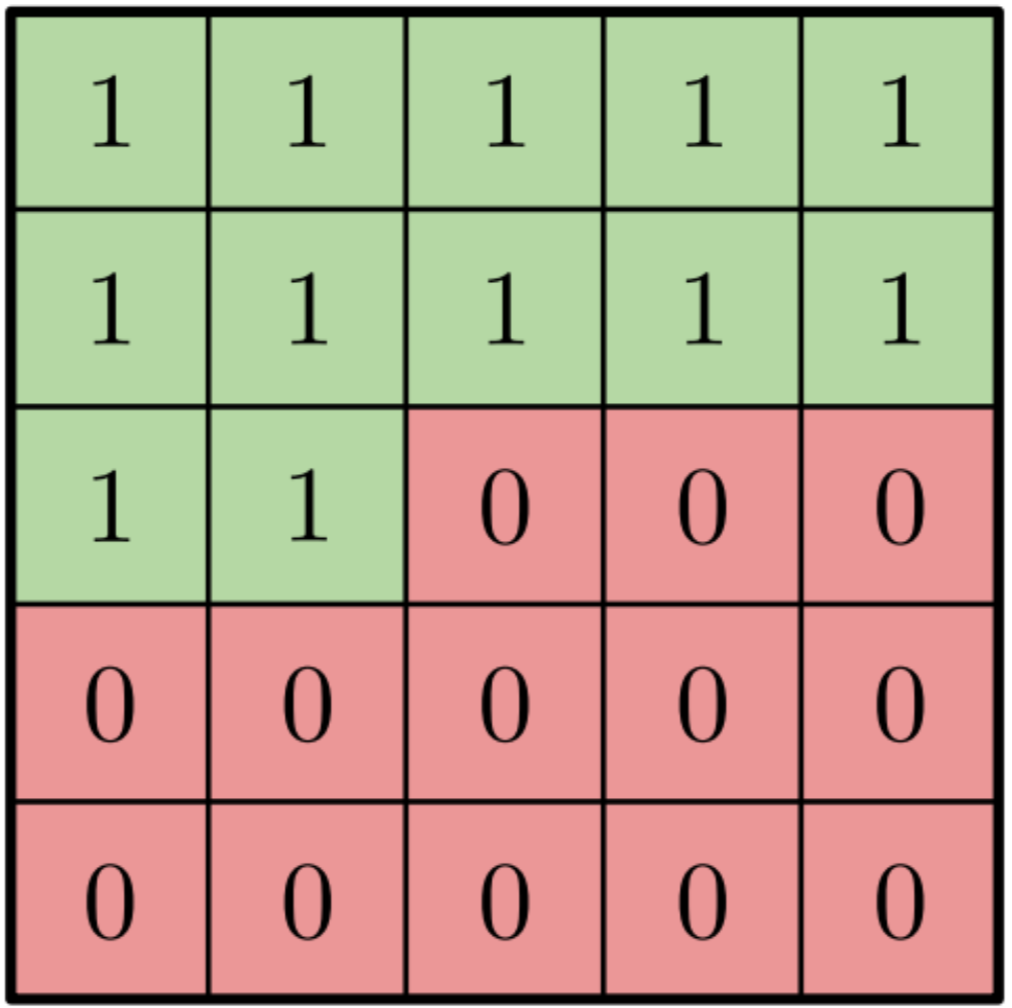
\includegraphics[width=0.6\textwidth]{figures/Autoregressive_Masked_Conv.png}
			\caption{Example mask for $5\times 5$ convolution}
		\end{subfigure}
		\hspace{2mm}
		\begin{subfigure}{0.32\textwidth}
			\centering
			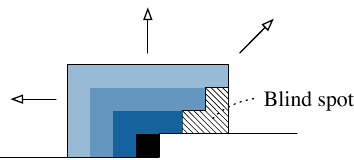
\includegraphics[width=\textwidth]{figures/Autoregressive_PixelCNN_blindspot_problem.png}
			\caption{Blindspot of PixelCNN}
		\end{subfigure}
		\hspace{2mm}
		\begin{subfigure}{0.32\textwidth}
			\centering
			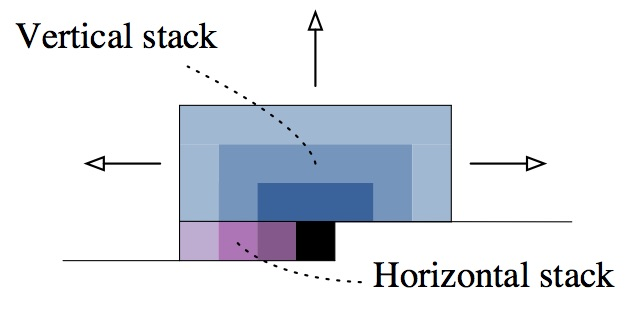
\includegraphics[width=\textwidth]{figures/Autoregressive_PixelCNN_blindspot.jpg}
			\caption{Solution to blindspot}
		\end{subfigure}
		\caption{Masked convolutions in PixelCNN}
		\label{fig:Autoregressive_PixelCNN}
	\end{figure}
	\item Problem: worse results than PixelRNN because of limited context and blind spot (cascaded convolutions ignore right upper part)
	\item Solution: use two convolutions, one vertical stack looking purely on the top part, and the horizontal stack looking to the right. Additionally, use gated convolutions (one half of the features go through tanh, the other through sigmoid)
	\item \textbf{PixelCNN++}: replace softmax with logistic mixture likelihood over 8 bits, use encoder-decoder architecture with skip connections
\end{itemize}
\subsubsection{PixelVAE}
\begin{itemize}
	\item Standard VAE with PixelCNN as decoder/generator
	\item However, generator is very powerful which can lead to the problem that it ignores the latent code, and just generates ``nice'' images
	\begin{figure}[ht!]
		\centering
		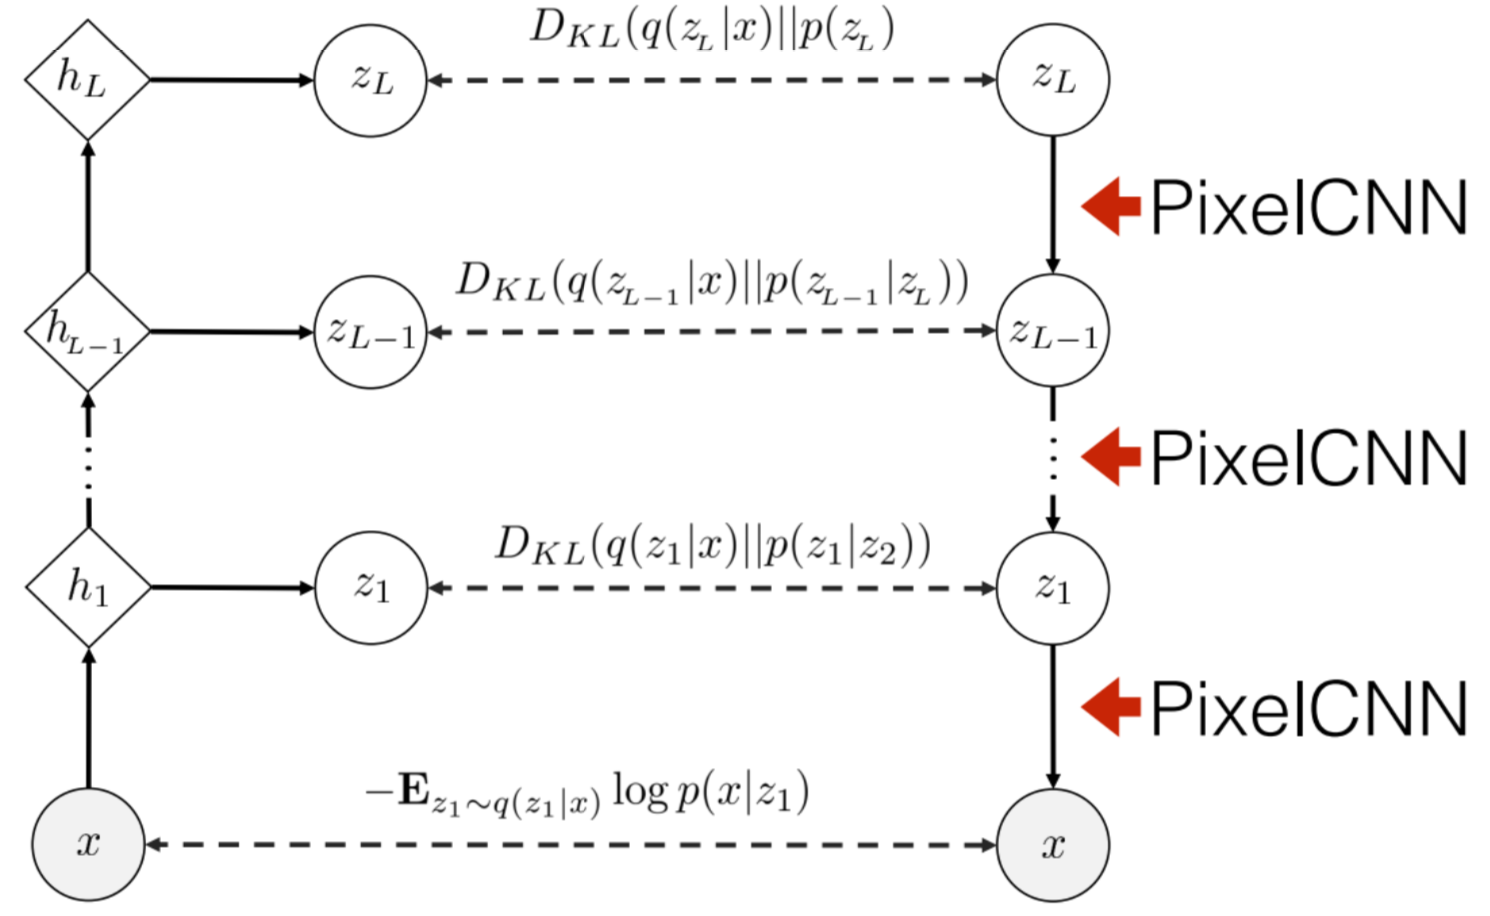
\includegraphics[width=0.3\textwidth]{figures/Autoregressive_PixelVAE.png}
		\caption{Architecture of a PixelVAE}
	\end{figure}
\end{itemize}
\section{Deep Reinforcement Learning}
\subsection{Fundamentals of Reinforcement Learning}
\begin{itemize}
	\begin{figure}[ht!]
		\centering
		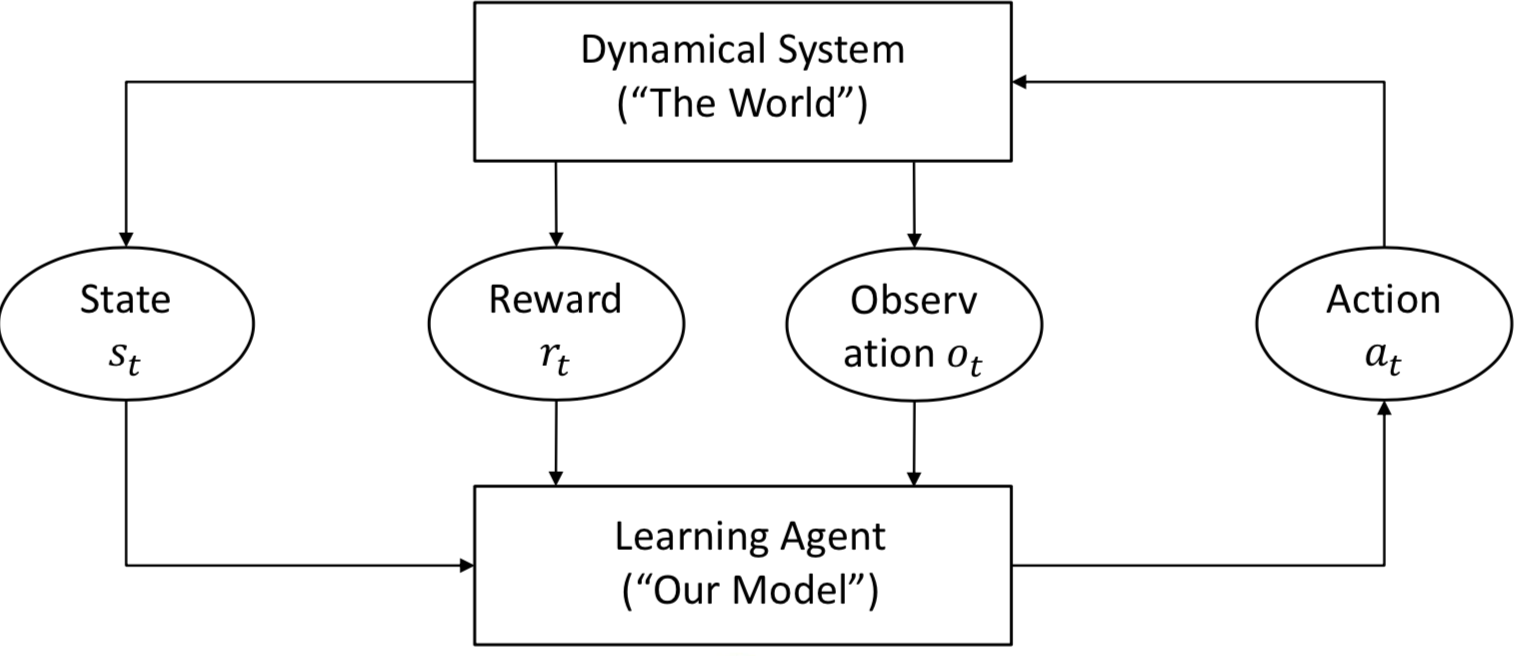
\includegraphics[width=0.4\textwidth]{figures/RL_basic_concept.png}
		\caption{Interaction model between environment and agent}
	\end{figure}
	\item The \textbf{state} $s_t$ is the summary of all experience so far: $s_t = f(o_1, r_1, a_1, o_2, r_2, a_2, ..., o_t, r_t)$ ($o_i$ observable part of environment at time step $i$). If we have a fully observable environment, then $s_t = f(o_t)$.
	\item The \textbf{policy} of an agent determines its actions: $\pi\left(a_t|s_t\right)$. Can be deterministic or stochastic
	\item The \textbf{value function} is the expected total reward under policy $\pi$: $$q^{\pi}(s_t, a_t) = \mathbb{E}_{\pi}\left[r_{t+1}+\gamma r_{t+2} + \gamma^2 r_{t+3} + ... | s_t, a_t\right]$$
	$\gamma$ as discount factor as we are most certain about close rewards and sometimes are more interested in immediate rewards
	\item \textbf{Bellman equation} for value function:
	$$q^{\pi}(s_t, a_t) = \mathbb{E}_{s', a'}\left[r + \gamma q^{\pi}\left(s', a'\right) | s_t, a_t\right] = \sum_{s'} p(s'|s_t,a_t)\cdot \left[r(s', a_t, s_t) + \gamma \sum_{a'} \pi(a'|s') \cdot q^{\pi}\left(s', a'\right) \right]$$
	\item The optimal value function is therefore $q^{*}(s_t,a_t) = \max_{\pi} q^{\pi}(s_t,a_t) = r_{t+1} + \gamma \max_{a_{t+1}}$
	\item The \textbf{environment} can be modeled by the agent (learned from experience), and used for planning and look ahead. This can be for example a simulator
\end{itemize}
\subsection{Deep RL approaches}
\subsubsection{Value-based approaches}
\begin{itemize}
	\item Try to learn value function $q^*$ to get the optimal policy $\pi^*$
	\item The input to such models is usually the state, which should be as raw as possible (e.g. image frames). We can either add the action to the input and let the network predict its Q-value, or predict Q-values for all possible actions (second is faster and simpler)
	\begin{figure}[ht!]
		\centering
		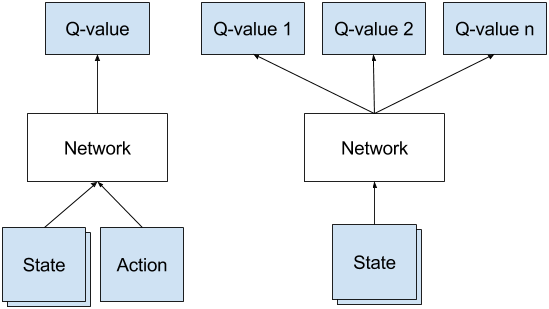
\includegraphics[width=0.4\textwidth]{figures/RL_deep_QLearning.png}
		\caption{Modeling of Q-value predictions}
	\end{figure}
	\item Optimization by SARSA-like loss:
	$$\mathcal{L} = \mathbb{E}\left[\left(r + \gamma \max_{a_{t+1}} q(s_{t+1}, a_{t+1}, \theta) -q(s_{t}, a_{t}, \theta) \right)^2\right]$$
	\item For the gradients, we assume that the bootstrapped max value is fixed:
	$$\pd{\mathcal{L}}{\theta} = \mathbb{E}\left[-2\cdot \left(r + \gamma \max_{a_{t+1}} q(s_{t+1}, a_{t+1}, \theta) -q(s_{t}, a_{t}, \theta) \right) \cdot \pd{q(s_{t}, a_{t}, \theta)}{\theta}\right]$$
	\item Optimize with SGD by sampling one action and state, calculate q-values for all possible future actions, and use the maximum as bootstrap goal
\end{itemize}
\subsubsection{Stability problems}
\begin{itemize}
	\item As we bootstrap, the target is always changing $\Rightarrow$ policy changes fast, can lead to oscillations
	\item The sequential data breaks the iid assumption on which SGD relies
	\item The scale of Q-values is not easy to control, and is very task dependent $\Rightarrow$ gradients are unstable and can be either too large or too small
	\item \textbf{Improving stability}
	\begin{itemize}
		\item \textit{Experience replay}: store memories of $\langle s, a, r, s'\rangle$ (with e.g. a $\epsilon$-greedy policy) in a dataset, and sample batches from there to train on. Breaks temporal dependency and helps SGD by i.i.d.
		\item \textit{Freezing target}: instead of having a moving target, we freeze the $Q$ network every $K$ iterations, and use that to generate our targets (Q-targets come now from a bit older network parameter setting, but is steady over $K$ iterations). Avoids oscillations
		\item \textit{Clipping rewards}: Normalize or clip rewards to be in range $[-1,+1]$ or any other stable range. Prevents unknown scales of $Q$
		\item \textit{Skipping frames}: a light version of experience replay is skipping $N$ frames between two data points to avoid too strong temporal dependency (two consecutive frames are very similar)
		\item \textit{Exploration vs Exploitation}: use a $\epsilon$-greedy policy with annealing temperature. In the beginning, we will focus on exploration while slowly converging to exploitation
	\end{itemize}
\end{itemize}
\subsubsection{Policy-based approaches}
\begin{itemize}
	\item Try to learn the optimal policy $\pi^*$ directly from experience (parameterized policy $\pi_w(a_t|s_t)$)
	\item Avoids learning the $q$ values which are hard for continuous action spaces, and tend to oscillate because of bootstrapping
	\item Training steps
	\begin{enumerate}
		\item Determine Q-value for current policy by running a simulation:\\ $q^{\pi_w}(s_t, a_t) = \mathbb{E}\left[r_t + \gamma r_{t+1} + \gamma^2 r_{t+2} + ... | \pi_{w}\right]$
		\item Maximize q-values as loss function. 
		\begin{enumerate}
			\item If policy is deterministic:
			$$\pd{\mathcal{L}}{w} = \mathbb{E}\left[\chain{q^{\pi}(s,a)}{a}{w}\right]$$
			\item If policy is stochastic:
			$$\pd{\mathcal{L}}{w} = \mathbb{E}\left[\pd{\log \pi^{w}(a|s)}{w} q^{\pi}(s,a)\right]$$
		\end{enumerate}
	\end{enumerate}
	\item Asynchronous Advantage Actor-Critic
	\begin{itemize}
		\item Learn both policy and value function
		\item Multiple agents that simultaneously interact with (copy of) environment and learn
		\item \textit{Advantage estimates}: Use the learned value function to compare to your actually gained $q$ value. Loss is therefore higher if unexpected things happen $\Rightarrow$ exploration
	\end{itemize}
	\begin{figure}[ht!]
		\centering
		\begin{subfigure}{0.45\textwidth}
			\centering
			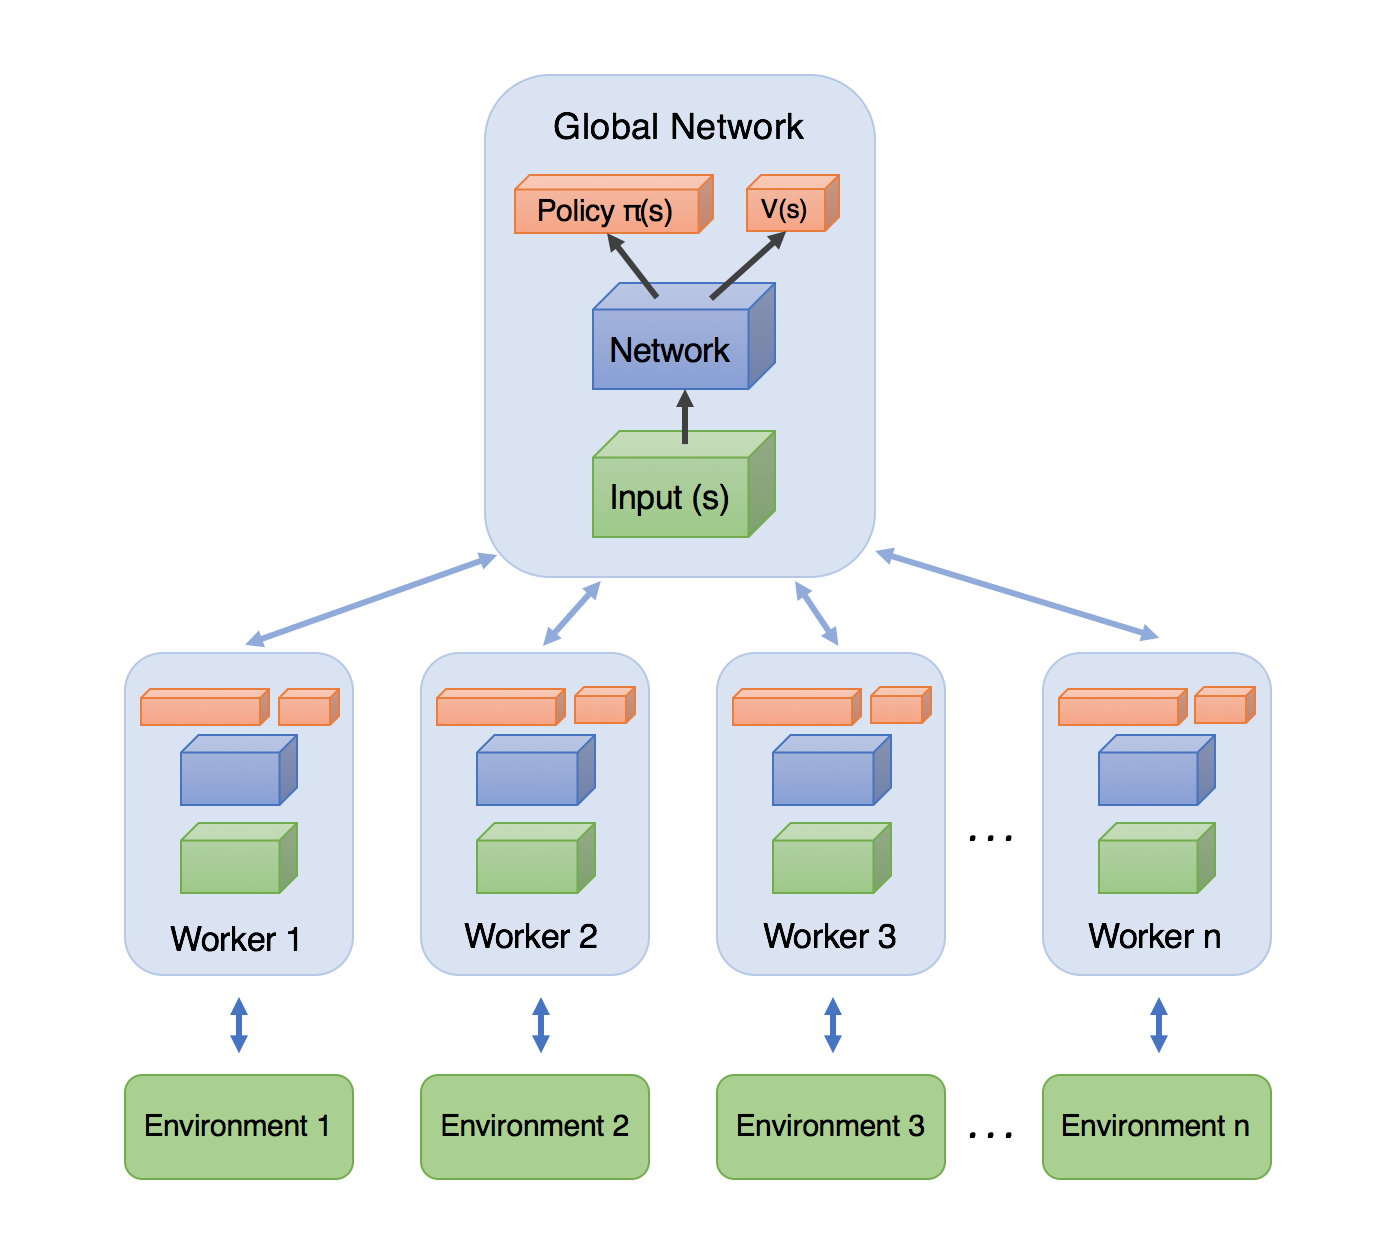
\includegraphics[width=0.8\textwidth]{figures/RL_A3C_multiple_workers.png}
		\end{subfigure}
		\begin{subfigure}{0.45\textwidth}
			\centering
			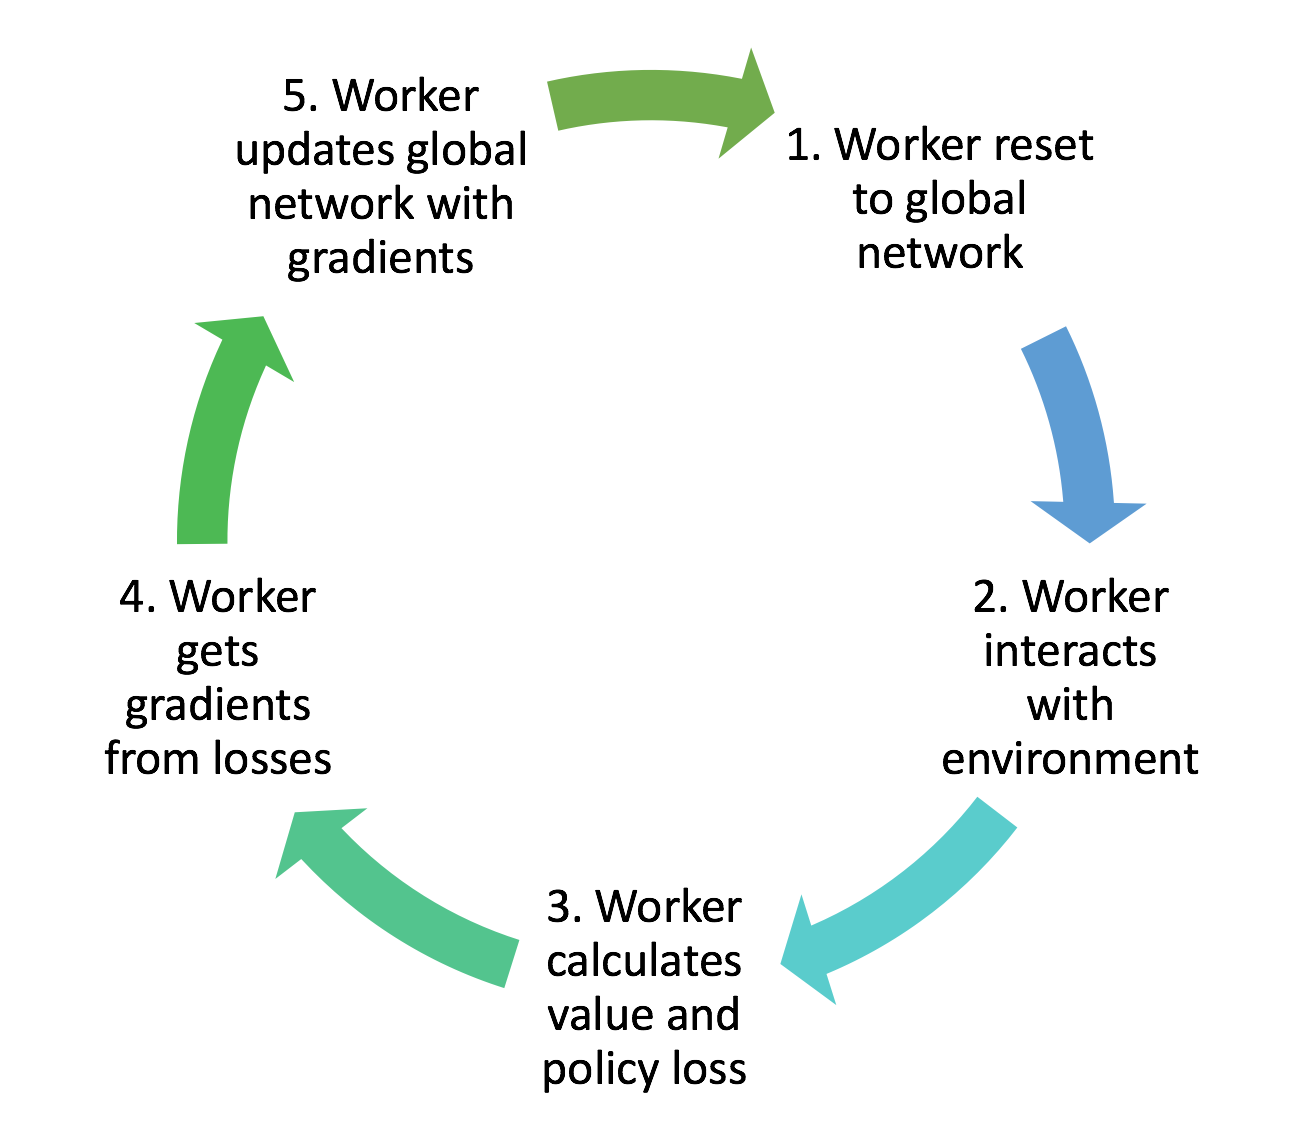
\includegraphics[width=0.8\textwidth]{figures/RL_A3C_cycle.png}
		\end{subfigure}
		\caption{Schematic overview of A3C}
		\label{fig:RL_A3C}
	\end{figure}
\end{itemize}
\subsubsection{Model-based approaches}
\begin{itemize}
	\item Try to model the environment to be aware of rules etc. 
	\item Example: AlphaGo relies on Tree-Search guided by CNNs. We use two policy networks to play against each other, and one value network that predicts the value function of a state
\end{itemize}
\appendix
\newpage
% \section{Neural Network Zoo}

\begin{figure}[ht!]
	\centering
	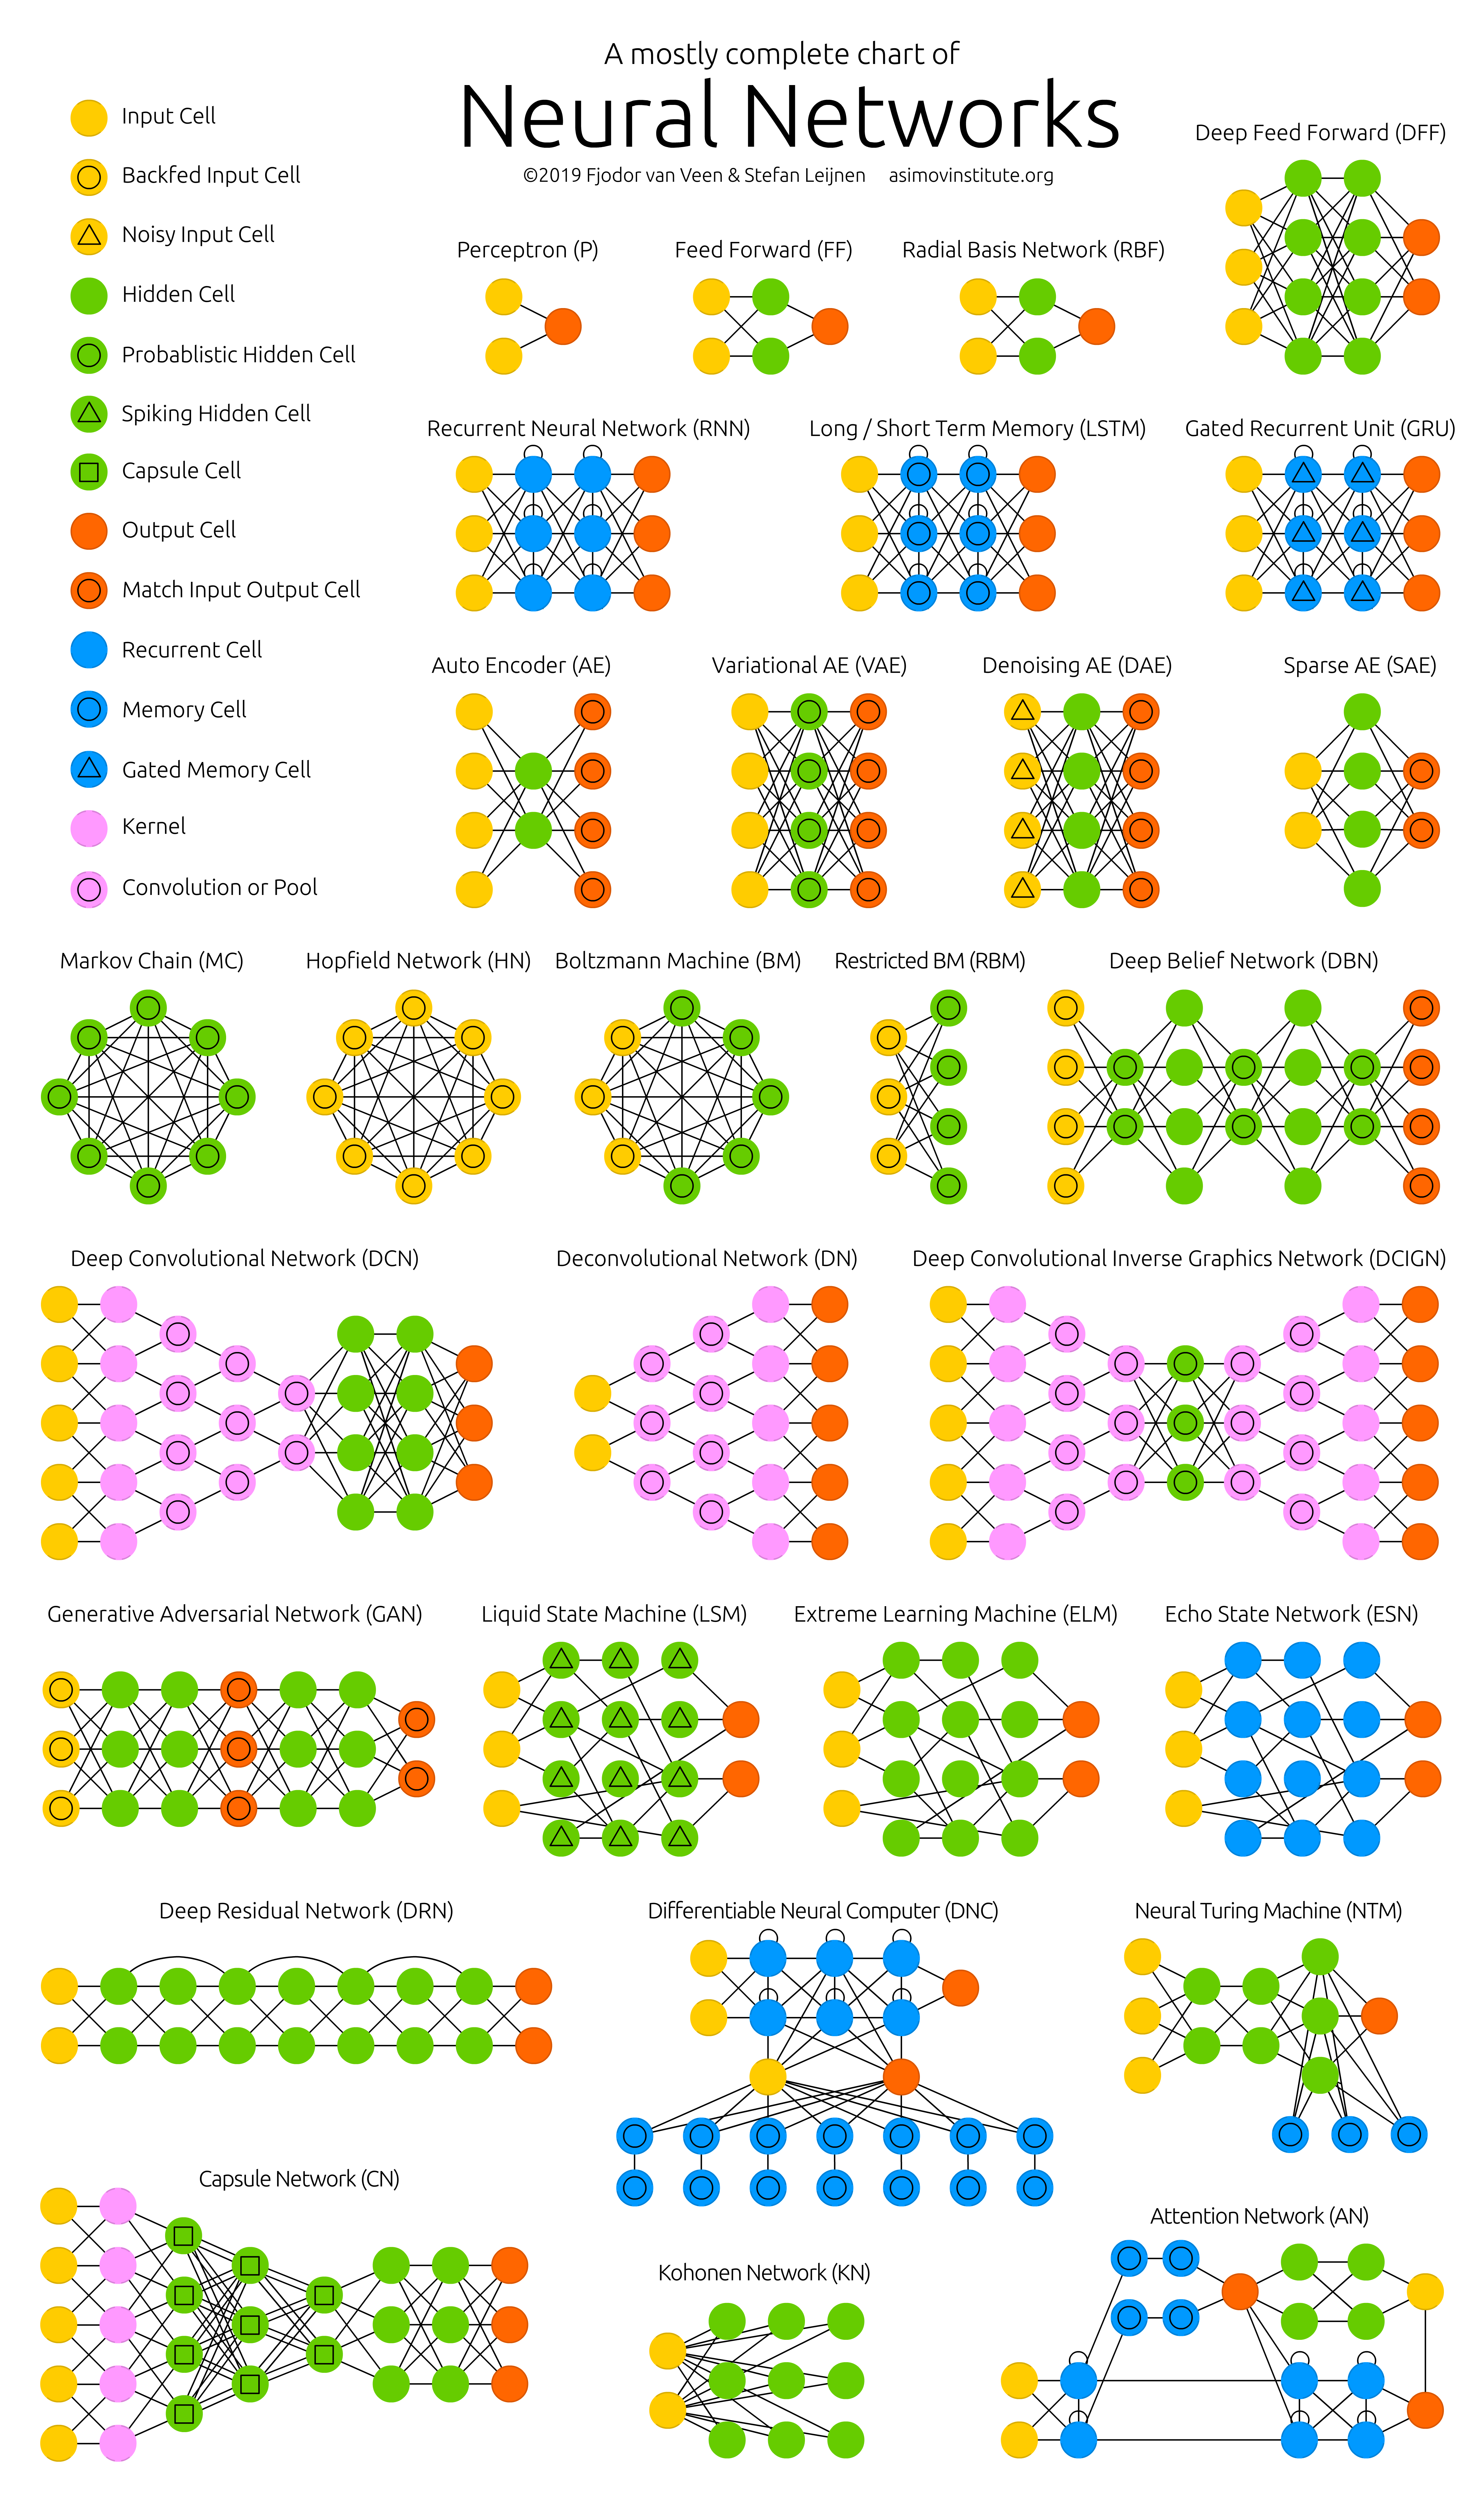
\includegraphics[width=0.9\textwidth]{figures/NN_Zoo_High.png}
\end{figure}

\end{document}